\documentclass
  [
  paper=a4,             % Papiergr��e
  fontsize=11pt,        % Basisschriftgr��e in Punkt
  DIV=calc,             % Autom. Berechnung eines DIV-Werts / manuell: Bereich 6 (gro�e)...15 (kleine R�nder)
  %twoside=true,         % ein-/zweiseitiges Layout (false, true)
  open=right,           % Kapitel nur auf rechter Seite beginnen (bei twoside=true)
  parskip=false,        % Abs�tze mit Zwischenraum (half, auch full = gr��erer Abstand)
  listof=numbered,
  bibliography=totocnumbered,
  %fleqn,               % Formeln linksb�ndig setzen
  %BCOR4mm,             % Bindekorrektur (zus�tzl. innerer Rand)
  ]
  {scrreprt}            % Dokumentklasse

\usepackage[english,ngerman]{babel}         % Neue deutsche Silbentrennung / Sprachpaket
\usepackage[latin1]{inputenc}               % deutsche Tastatureingabe
\usepackage[headsepline,footsepline]{scrpage2}  % Kopf- und Fu�zeilen mit Linien

\usepackage{graphicx,float}					% Einbinden von Grafiken und Bildern
\usepackage{amsmath, amssymb, amstext, amsfonts}	% Mathematikpakete
\usepackage{units}							% Angabe von Einheiten mit $\unit[220]{kV}$

\usepackage{booktabs}						% erweiterte Befehle f�r Tabellen
\usepackage{tabularx}						% Tabellen gleicher Gesamtbreite anlegen (Spaltenbreite kann variabel sein)
\usepackage{multirow}						% Mehrere Zellen miteinander verbinden
\usepackage{colortbl}						% Zeilen oder Zellen in Tabellen f�rben

\usepackage{xspace}                         % Zur Definition von Befehlen f�r mehrgliedrige Abk�rzungen ben�tigt
\usepackage{setspace}						% Seitenr�nder? und Zeilenabstand �nderbar
  %\onehalfspacing							% 1,5-facher Zeilenabstand
\usepackage{color}							% Farben festlegen
\usepackage[absolute]{textpos}              % Absolute Positionierung erm�glichen f�r Titelseite
\usepackage{ifthen}

\usepackage[fixlanguage]{babelbib}			% Zitieren (Quellen referenzieren) / Literaturverzeichnis
  \bibliographystyle{babplain}              % Zitierstil (babplain, babplai3, babalpha, babunsrt, bababbrv, bababbr3)

\usepackage{pdfpages}                       % pdf-Dokumente (teilweise) einbinden

\def\langencond{english}
\def\langdecond{ngerman}
\def\pglay{twoside}
% EOF 
\def\lang{english}         %%% choose your document language here: 'ngerman' OR 'english'
%\def\pagelayout{twoside}   %%% choose single or twosided layout
\usepackage[latin1]{inputenc}
\usepackage[table]{xcolor}
\usepackage{listings}
\usepackage{physics}
\usepackage{pdflscape}
\usepackage{pdfpages}
\usepackage{graphicx}
\usepackage{cclicenses}
\usepackage{amsmath}
\usepackage{ragged2e}
\usepackage{tikz}
\usepackage{array, booktabs, caption}
\usepackage{makecell}
\usepackage{longtable}
\usepackage{multicol}
\usepackage{siunitx}
\usepackage{nomencl}
\usepackage{tikz}
\usetikzlibrary{fit}
\usetikzlibrary{calc,fit,arrows}
\usetikzlibrary{shapes,arrows}
\usetikzlibrary{calc,positioning,shapes.geometric}
\usepackage{enumitem}
\usepackage{amsmath,amsfonts,amssymb}
\usepackage{tikz}
\usetikzlibrary{automata,positioning}
\makenomenclature 
\newcommand{\inch}{\ensuremath{\,\textrm{in}}}
\renewcommand\theadfont{\bfseries}
\usetikzlibrary{shapes,shapes.multipart,shadows,arrows,shapes.misc}
\usepackage{color} %red, green, blue, yellow, cyan, magenta, black, white
\definecolor{mygreen}{RGB}{28,172,0} % color values Red, Green, Blue
\definecolor{mylilas}{RGB}{170,55,241}
\newenvironment{rcases}
  {\left.\begin{aligned}}
  {\end{aligned}\right\rbrace}
        %%% choose your document language here: 'ngerman' OR 'english'
%\def\pagelayout{twoside}   %%% choose single or twosided layout

%===========================================%
% zus�tzliche Pakete hier einbinden!!!      %
%-------------------------------------------%



%-------------------------------------------%
% zus�tzliche Pakete oberhalb einbinden!    %
%===========================================%

%===========================================%
% Dokument-Metadaten (bitte ausf�llen!)     %
%-------------------------------------------%

\def\author{Md. Rakibul Islam}
\def\subject{ Adapting semantic perception for long-term manipulation using perceptual episodic memorie }
\def\tutorA{Ferenc Balint-Benczadi}
\def\tutorB{~}
\def\examinerA{Prof. Dr.-Ing. Kai Michels}
\def\examinerB{Prof. Michael Beetz}

\ifx\lang\langencond
  \def\title{Master Thesis}
  \def\keywords{keyword 1, keyword 2}
  \def\tutorhead{Tutor:}
  \def\examinerheadA{Examiner:}
  \def\examinerheadB{}
  \def\textlanguage{en-us}
\fi
\ifx\lang\langdecond
  \def\title{Projekt-/Studienarbeit}
  \def\keywords{Stichwort 1, Stichwort 2}
  \def\tutorhead{Betreuer:}
  \def\examinerheadA{Pr\"ufer:}
  \def\examinerheadB{}
  \def\textlanguage{de-1996}
\fi

\def\submissiondate{\today}
\def\editorsoftware{WinEdt 6.0}

%-------------------------------------------%
% Dokument-Metadaten Ende                   %
%===========================================%

\usepackage[pdfborder={0 0 0}]{hyperref}    % Hyperlinks/Metadaten - unbedingt als letztes Paket einbinden!

\ifx\pagelayout\pglay
  \KOMAoptions{twoside}
\fi

%========================================================================================%
%========================================================================================%

\graphicspath{{bilder/}}  % Suchpfad f�r Bilder

\setlength{\TPHorizModule}{1cm}  % Einheit f�r absolute horiz. Positionierung definineren
\setlength{\TPVertModule}{1cm}  % Einheit f�r absolute vert. Positionierung definineren
\renewcommand{\chapterpagestyle}{scrheadings}  % Kopf- und Fu�zeile auch auf Kapitelanfangsseiten


%===========================================%
% Kopf- und Fu�zeile formatieren            %
%-------------------------------------------%

\pagestyle{scrheadings}
  \automark[section]{chapter}
  \definecolor{iat_red}{rgb}{0.8,0,0}
  \setheadsepline{1.2mm}[\color{iat_red}]

\ihead{\textsf{\headmark}}
\chead{\textsf{}}
\ohead{
\includegraphics[width=1.14cm]{iat_logo}}

\ifoot[]{\textsf{}}
\cfoot[]{\textsf{}}
\ofoot[\textsf{\pagemark}]{\textsf{\pagemark}}

%-------------------------------------------%
% Kopf- und Fu�zeilenformatierung Ende      %
%===========================================%



%========================================================================================%
%========================================================================================%



%===========================================%
% Benutzerbefehle (Neudefinitionen)         %
%-------------------------------------------%

\newcommand{\zB}{\mbox{z.\,B.}\xspace}
\renewcommand{\dh}{\mbox{d.\,h.}\xspace}
\newcommand{\Dh}{\mbox{D.\,h.}\xspace}
\newcommand{\tbs}{\textbackslash}           % Backslash einf�gen (Abk�rzung des Befehls)
\newcommand{\bs}{\boldsymbol}               % fett + kursiv z.B. f�r Matrizen oder Vektoren (Abk�rzung)

%-------------------------------------------%
% Benutzerbefehle (Neudefinitionen) Ende    %
%===========================================%




%===========================================%
% Dokument-Metadaten                        %
%-------------------------------------------%
\hypersetup   % Meta-Daten (bitte eingeben)
  {
  pdftitle      ={\title},
  pdfauthor     ={\author},
  pdfsubject    ={\subject},
  pdfcreator    ={\editorsoftware},
  pdfproducer   ={pdfLaTeX},
  pdfkeywords   ={\keywords},
  pdflang       ={\textlanguage}   % Language-identifier (RFC 3066) (de-1996, en-US, en-GB)
  }

\hypersetup   % Ansichtsoptionen
  {
  pdfstartview    ={Fit},             % Startansicht im Viewer
  pdfcenterwindow ={true},            % Startansicht im Viewer
  pdfpagelayout   ={SinglePage},      % Layout im Viewer (TwoColumnRight, TwoPageRight, OneColumn, SinglePage)
  colorlinks      ={false}            % Hyperlinks nicht einf�rben
  }
%-------------------------------------------%
% Dokument-Metadaten Ende                   %
%===========================================%

% EOF 

%%%%%%%%%%%%%%%%%%%%%%%%%%%%%%%%%%%%%%%%%%%%%
%%%%%%%%%%%%%%%%%%%%%%%%%%%%%%%%%%%%%%%%%%%%%
%%%                   %%%%%%%%%%%%%%%%%%%%%%%
%%%  Dokument-Anfang  %%%%%%%%%%%%%%%%%%%%%%%
%%%                   %%%%%%%%%%%%%%%%%%%%%%%
%%%%%%%%%%%%%%%%%%%%%%%%%%%%%%%%%%%%%%%%%%%%%
%%%%%%%%%%%%%%%%%%%%%%%%%%%%%%%%%%%%%%%%%%%%%
\begin{document}
\ifx\lang\langencond
  \selectlanguage{english}
\fi
\ifx\lang\langdecond
  \selectlanguage{ngerman}
\fi

\begin{titlepage}
  \hbox{}
  \begin{textblock}{21}(0,0)

  % Kopfzeile
  \begin{figure}[t]
    \centering
	
\includegraphics[width=\textwidth]{iat_head}
  \end{figure}
  \vspace{24.67cm}
  \begin{figure}[b]
    \centering
	
\includegraphics[width=\textwidth]{iat_foot}
  \end{figure}
  \end{textblock}


  \begin{textblock}{14}(3.5,7)
    \centering
    {\large\bfseries
      \title
    \par}
    \vspace{1.2cm}
    {\linespread{1.1}\huge\sffamily\bfseries
      \subject
    \par}
    \vspace{1.2cm}
    {\Large
      \author
    \par}
    \vspace{0.5cm}
    \submissiondate
  \end{textblock}


  \begin{textblock}{14}(3.5,21)
    \centering
    \begin{minipage}[t]{0.4\textwidth}
      \begin{flushleft} \large
        \underline{\tutorhead}       \\[0.25em]
        \tutorA                     \\[0.25em]
        \tutorB
      \end{flushleft}
    \end{minipage}
    \hspace{0.1\textwidth}
    \begin{minipage}[t]{0.4\textwidth}
      \begin{flushleft} \large
        \underline{\examinerheadA}   \\[0.25em]
        \examinerA                  \\[1em]
        \underline{\examinerheadB}   \\[0.25em]
        \examinerB
      \end{flushleft}
    \end{minipage}

  \end{textblock}


  \thispagestyle{empty}
\end{titlepage}


\cleardoublepage
\thispagestyle{empty}



%%%%%%%%%%%%%%%%%%%%%%%%%%%%%%%%%%%%%%%%%%%%%
%%%  ABSTRACT - if requested                %
%%%-----------------------------------------%
\cleardoublepage
~\\
\vspace{1cm}

\noindent{\Large\textbf{\textsf{Copyright declaration}}}\\[2em]
I hereby declare that I have finished my thesis without any external help, and that I have not used any sources other than the ones I have indicated.\\[1em]
All passages, taken literally or meaningfully from the publications, I have indicated as such, with reference to the sources.\\[1em]
The thesis will not be modified after submission.\\[3em]
Date: \rule{3.2cm}{0.4pt} \hspace{0.6cm} Signature: \rule{5.4cm}{0.4pt}

\cleardoublepage
\thispagestyle{empty}
\chapter*{Acknowledgement}
It is the best time in my life to show gratitude towards who are constantly with me such as the almighty God and my parents. I am grateful to my tutor Ference to guide me during the hole thesis work and his guidance helps me to finish the work successfully. Whenever I need any documents in my entire master studies life, I always go to Prof. Dr.-Ing. Kai Michels and he never disappointed me. I am greatly grateful to him to allow me to do my master thesis outside department-1. I want to take the opportunity to thank also Prof. Michael Beetz who allowed me to work in this fascinating area of research.


\chapter*{Abstract}
Robots operating in human environment have to deal with complex manipulation tasks. For this robot needs to equipped with perceptual capabilities. One of the most important perceptual capability is how robot recognize and learn about novel objects from its surroundings.
\\\\
The evaluation of this capability can be achieved by generating the perceptual episodic memory during the execution of a task. The perceptual episodic memory has great impact in robotic perception, because it can enable robot to relive past events and learn from them.
\\\\In the manipulation task robot has to perceive and classify different objects, which contains novel objects also. To classify objects, the classifier should be trained with large dataset. The dataset contains the objects or object's group, which must be present in robot working environment. In this thesis work, we used two datasets. One is RGBD dataset from university Washington and the other one is kitchen environment dataset from Institute for artificial intelligent.
\\\\Since object classification results is highly influenced by the algorithms for extracting feature from the images. We develop a tool for extracting feature and split the feature into train and test date. As feature extraction algorithm, we use CNN and VGG16 to get the object class and VFH and CVFH for object's shape.
\\\\We use popular machine learning algorithm such as random forest, support vector machine, k-nearest neighbor and gradient boost tree. We trained the classifier and evaluate its performance by using both the test and data coming from manipulation task.

%%%-----------------------------------------%
%%%  ABSTRACT ends here                     %
%%%%%%%%%%%%%%%%%%%%%%%%%%%%%%%%%%%%%%%%%%%%%

\cleardoublepage
\tableofcontents    % table of contents
\cleardoublepage

%%%%%%%%%%%%%%%%%%%%%%%%%%%%%%%%%%%%%%%%%%%%%
%%%  DOCUMENT begins here                   %
%%%-----------------------------------------%
\chapter{Introduction}
Semantic perception consists of meaning full informations such as object names, it's geometric informations like object's position and orientation information, understanding the relations between them from the senor data. Different algorithms are used to generate  and attach the semantic perceptions to sensor data. Using this semantic perceptions robot perceive about the surroundings world in front of it. Semantic informations also help us to evaluate a robot's limitation to perceive the objects in different conditions. So it important to store them. 
\\\\ In the context of robotic perception, perceptual episodic memory is used to store the semantic perception. Episodic memory helps researcher to get all the necessary informations about a manipulations task that a robot has performed. So the researcher can understand if there is any mistake happened during the task execution. It helps to find the different relations between the different semantic perceptions. As a result, these relations can be used to build new learning problems, which can improve robot perception.  
\section{Motivation}
For a robot performing human like perception in general is very difficult and need to cope with many algorithms. Let's consider a simple pick and place task that a robot performing in a kitchen environment. Even for this simple task, the properties of objects vary frequently and therefore the different algorithmic approaches are needed for detecting them. For example, detecting shiny cutlery from a drawer is handle very differently then detecting a cereal box from the shelf. Even this problem get more harder in different lightening condition. Moreover, During the task execution phase, false detection may occurs without noticing.To consider these problems, the perception for long-term manipulation task such ones mentioned above, needs to address on a system level.
  

\section{Goal}
In this thesis work, we build a perception system using the open source perception framework \textbf{RoboSherlock} \cite{beetz2015robosherlock} with active memory. The developed system will be rapped with machine learning algorithms, which classify the objects during the manipulation tasks and also consists of tool to logged task's results in the active memory and query the memory. We also focus on finding the answers of the following questions: \\
From how far a robot can detect an object perfectly and that is the angel between the robot's camera and the object at that moment. 
\\\\
We mainly focus on finding the answers of the following questions: \\
From how far a robot can detect an object perfectly and that is the angel between the robot's camera and the object at that moment. And how real world data can be use to classify using turn table data.  In order to be able to answer this question we need to store the semantic perception as episodic memory.  Everything the robot 'see' during the execution of a task is logged as episodic memories. To achieve our goal, use use Robosherlock a robotic perception framework. The frame work provides perception capabilities for mobile robots performing long-term manipulation task in kitchen environment. From this frame work we use different components called annotator or expert algorithm to generate object hypothesis and annotates the object hypothesis with different kind of semantic perception information from row sensor data (images). We also build tool for extracting features from input datasets( collections of depth and RGB images) and annotators to work with popular machine learning algorithms like support vector machine, random forest, k-nearest neighbor and gradient boost tree classifier. We evaluate the algorithms or classifiers performance using the open source datasets form Uni washington and the kitchen environment datasets from Institute for artificial intelligent. 

In this thesis work we consider that the robot is working in the kitchen environment and the task of the robot is like pick and place of the object. We use Washington university dataset \cite{lai2011large} and kitchen environment dataset from institute for artificial intelligent. Both datasets are created by taken image of different objects using a turn table with and angle difference 30 degree. We use popular supervised machine learning algorithms like support vector machine, random forest, k-nearest neighbor, gradient boost tree to create the trained model in order to classify the data which is coming from real world robot manipulation task. Before classify the real world data we cross validate our trained model using the test data and  evaluate the performance of the classifiers. The real world data is recorded during the robot manipulation task and put it into a database. The real data is row sensor date and consider as unstructured data. In oder to classify this data we need structure informations from the data. The perception framework robosherlock provide the expert algorithms or annotators which generate structured object hypothesis and annotate the hypothesis with different semantic information. As our interest 
to classify the real world data so we need to add class label with this objects hypothesis.
So we build the classifier as the framework annotator and run together with other annotators in pipe line. This ensemble of annotators is called analysis engine. At this moment our real world data is fit for evaluation because it has enough ground truth informations. The trained model which has been created from the dataset consists of all the possible objects, which are found in a kitchen environment. We again run the analysis engine and logged all the output data into another database. The database contains all semantic perceptions which added to data during the running of the pipe line and database is now consider as the episodic memory. This memory has great impact in robotic perception.
As we use the mongoDB database which provide the tools and software to query the database and generate new learning problems which improve robotic perceptions. The over of whole work is presented by a flow charts.

\section{Related Work}
In this chapter we are going to discuss the components of our work which are related to other's work.
\\
In \cite{marton2013ensembles} authors described how to compute feature from image data using different feature extractions algorithms (especially VFH) and classify them using different machine learning algorithms such support vector machine. Also showed different techniques to ensemble classifiers, which would improved the classification accuracy. 
\\\\ Shape of a object is very good source to classify objects in different categories. object shape can be found from RGB-D images. VFH (View Point Feature Histogram) \cite{rusu2010fast} is very prominent algorithm, which is used to calculates descriptor from depth image. It calculates histogram based on the relative angles between the surface normals of the objects to the normal viewpoint direction of the sensor. It was developed to be robust again noise, which is common in depth image sensors. Based on VFH another algorithm called CVFH(Cluster Viewpoint Feature Histogram) \cite{aldoma2011cad} is calculated. It works on object's cluster in the depth image. It useful for object recognition and pose estimation of rigid objects.
\\\\Memory for robot is described in literatures \cite{niemueller2013towards}, \cite{niemueller2013life} \cite{oliveira2014perceptual}.Their authors described how to store data and learn form perceptual episodic memory. For working with the data they use to separate memory locations, one for perceptual memory and the second one is for semantic memory. They use non-relational database called mongoDB as central location for perceptual memory.
\\\\A general over view of this thesis topic "Adapting semantic perception using perceptual episode memory" is very much similar to approach describe in literature \cite{balint2017storing}, where authors showed how episodic memory can be used to retrospect a robot manipulation task and query the memory to generate new supervised learning problem.
\section{Overview}
The structure of this paper is as follows: Related work is described in Section II. Next, we give a brief description of our system architecture in Section III. We discuss our surface normal and segmentation algorithm in Section IV followed by a discussion of the Viewpoint Feature Histogram in Section V. Experimental setup and resulting computational
and recognition performance are described in Section VI. Conclusions and future work are discussed in Section VII
The project report is organized ino six chapters. Chapter 2 deals with the theoretical background, chapter 3 describes the existing MATLAB model, chapter 4 covers the reprogrammed model in C++, chapter 5 includes program testing and the final chapter contains the conclusion.
\chapter{Feature Extraction Algorithm}
\section{descriptor}
When we work with RGB-D depth image, we calculate descriptors. 3D feature is called descriptors. They are more complex (and precise) signatures of a point, that encode a lot of information about the surrounding geometry. The purpose is to unequivocally identify a point across multiple point clouds, no matter the noise, resolution or transformations. Also, some of them capture additional data about the object they belong to, like the viewpoint (that lets us retrieve the pose). descriptors can be two types local descriptors and global descriptors. Local descriptors are computed for individual points that we give as input. They have no notion of what an object is, they just describe how the local geometry is around that point. Global descriptors encode object geometry. They are not computed for individual points, but for a whole cluster that represents an object. Because of this, a preprocessing step (segmentation) is required, in order to retrieve possible candidates.
Global descriptors are used for object recognition and classification, geometric analysis (object type, shape...), and pose estimation.
\subsection{Viewpoint Feature Histogram}
The VFH (Viewpoint Feature Histogram) is derived from the FPFH (First Point Feature Histogram). The VFH consists of two parts: a viewpoint direction component and an extended FPFH component. To calculate the first one, the object's centroid is computed, which is the point that results from averaging the X, Y and Z coordinates of all points. After that, the vector between the viewpoint (the position of the sensor) and the centroid is computed, and normalized. Finally, for all points in the cluster, the angle between their normal and this vector is calculated, and the result is binned into an histogram. The vector is translated to each point when calculating the angle cause it makes the descriptor scale invariant. The viewpoint direction component calculation is shown graphically in figure below.

\begin{figure}[H]
\centering
\includegraphics[width=0.6\textwidth]{figure/vfh_1}
\caption{a viewpoint direction component }
\end{figure}

The second component is calculated like as the FPFH that generates 3 histograms for the 3 angular features $ \alpha $, $\phi$ and $\theta$ as shown in fig below. 
\begin{figure}[H]
\centering
\includegraphics[width=0.6\textwidth]{figure/vfh_2}
\caption{a viewpoint direction component }
\end{figure}
It is measured between  between the viewpoint direction at the centroid and each of the normals on the surface. The bottom left part of the above Figure presents the selection of the Darboux frame and a graphical representation of the three angular features.
In detail, for a pair of 3D points ($p_{i}$, $p_{j}$) and their estimated surface normals ($n_{i}$, $n_{j}$) the set of normal angular deviations can be calculated as: 
\begin{align}
\begin{split}
\alpha = v \cdot n_{j} \\ 
\phi =u \cdot \dfrac{(p_{j}-p_{i})}{d} \\
\theta= arctan(w \cdot n_{j}, u \cdot n_{j})
\end{split}
\end{align}
where $u$, $v$, $w$ represent a Darboux frame coordinate system chosen at $p_{i}$. Then, the Point Feature Histogram at a patch of points $P = {p_{i}}$ with $i = {1,.....,n}$ captures all the sets of ($\alpha$, $\phi$, $\theta$) between all pairs of ($p_{i}$
, $p_{j}$) from $P$, and bins the results in a histogram. The resulting 4 histograms as 1 for the viewpoint component and other 3 for the extended FPFH component are concatenated to create the final VFH descriptor as shown in figure below. 

\begin{figure}[H]
\centering
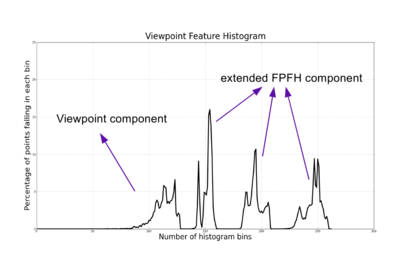
\includegraphics[width=0.9\textwidth]{figure/vfh_3}
\caption{VFH histogram }
\end{figure}


%%
%\begin{figure}[!tbp]
%  \centering
%  \begin{minipage}[b]{0.4\textwidth}
%    \includegraphics[width=\textwidth]{vfh_1}
%    \caption{Viewpoint component of the VFH}
%  \end{minipage}
%  \begin{minipage}[b]{0.5\textwidth}
%    \includegraphics[width=\textwidth]{vfh_2}
%    \caption{Extended FPFH component of the VFH}
%  \end{minipage}
%\end{figure}


% By default, the bins are normalized using the total number of points in the cluster. This makes the VFH descriptor invariant to scale.The PCL implementation computes an additional fifth histogram with the distances of the cluster points to the centroid (the Shape Distribution Component, SDC), increading the size of the output descriptor from 263 to 308. The SDC is taken from the CVFH descriptor that we will see in the next section, and makes the result more robust.
\section{Theoretical Background }
In this thesis work we are working with image data and find out the best classification algorithm, which classifies the data in the most precisely. As to work with the whole image is very costly, so we use algorithm to find the pixel points or features in the image, which can represent the corresponding image perfectly. Deep learning algorithms are very efficient and precise to describe the image features. Therefore, in our work we use convolution nural network (CNN) and visual geometric group (VGG16) as our features. For point cloud or 3D image, we use view point feature histogram and cluster viewpoint feature histogram algorithms. For classification there are a lots of algorithms available in Machine learning. Reviewing the literature, we are come up with the support vector machine (svm), random forest(RF), gradient boosting (GBT) and K-nearest neighbor algorithms. The descriptions about the algorithm and how these work are given bellow; 


\section{shape based object recognition}

\section{Feature}
When we process images, we can not work with hole image due to high computational cost. Instead of this, we find out some points by applying some characteristics using different algorithm in the image. These characteristics of the point is called feature, which can help us to differentiate one point from another point in image. We can tell a feature is optimal, if it satisfied the following criteria:
\\
\\
1.It must be robust to transformations: rigid transformations (the ones that do not change the distance between points) like translations and rotations must not affect the feature. Even if we play with the cloud a bit beforehand, there should be no difference.
\\\\It must be robust to noise: measurement errors that cause noise should not change the feature estimation much.
\\\\ It must be resolution invariant: if sampled with different density (like after performing downsampling), the result must be identical or similar.
\subsection{Convolution Neural Network}
\subsection{Visual geometric group}


\chapter{Learning Algorithm}
In general, any machine learning algorithm can be divided into one of the two major types called supervised and unsupervised learning. 

\begin{description}[leftmargin=*]
\item[Supervised learning]
In this learning, we are given a data set and we already know what our exact output should look like, considering the idea that there is a relationship between the input and the output. Supervised learning problems are again categorized into "regression" and "classification" problems. In a regression problem, we predict results within a continuous output, so we map input variables to some continuous function. In a classification problem, we predict results in a discrete output. In other words, we try to map input variables into discrete categories. Examples of Supervised Learning are Regression, Decision Tree, Random Forest, K-nearest neighbor, Logistic Regression etc.
\item[Unsupervised learning] This learning allows us to deal problems with very little or no idea what our results should look like. We try to derive structure from data where we don't necessarily know the effect of the variables. We can derive this structure by clustering the data based on the relationships among the variables in the data. In this algorithm, we do not have any target or outcome variable to predict or estimate. So there is no feedback based on the prediction results. Examples of unsupervised learning are K-means, Apriori algorithm etc.
\end{description}
 
In thesis thesis work we solely focus on supervised learning more precisely classification problem. There are a lot of supervised learning algorithms available to choose from. We pick most popular ones such as Support Vector Machine, Random forest, K-nearest Neighbor, Gradient boost tree for our data classification tasks. The details about how this algorithms work are described in the followings. 

\section{Support Vector machine}
Support vector machine is a complex and advanced machine learning algorithm. It works on labeled train samples (supervised learning) and outputs an optimal hyperplane which categorize 
novel samples. The algorithm tries to find the hyperplane that gives the largest minimum distance to the training samples. For better intuition of how the algorithm decide the optimal hyperplane, lets consider the following scenarios. Consider the image below which has two types of data, red and blue. Form the image it is clear that, there are many lines  possible lines to separate the blue and read data. 

\begin{figure}[H]
\centering
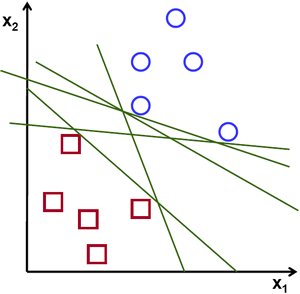
\includegraphics[width=0.4\textwidth]{figure/svm_basics1}
\caption{support vector machine }
\end{figure}

Therefore, we need a way to find out the best line to separate the data. The algorithm finds out some special data points from both types (in below figure filled blue and read rectangle points) which are very close to each others. These data points are called support vectors and the lines pass through them are called support planes (doted green lines).    

\begin{figure}[H]
\centering
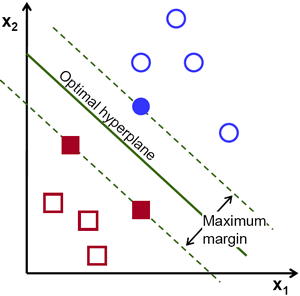
\includegraphics[width=0.4\textwidth]{figure/svm_1}
\caption{support vector machine }
\end{figure}
Then the algorithm finds the optimal hyperplane (bold green line), which passes thorough the maximum margin distance from both of the support planes. To get the maximum margin is an optimization problem. So far we consider the data which are linearly separable. 
\\\\Lets consider the following figure, where data can not be linearly separable. So svm uses a technique called kernel trick. The kernel trick is a special function, which maps the train samples from lower dimensional feature space to higher dimensional  feature space. 

\begin{figure}[H]
\centering
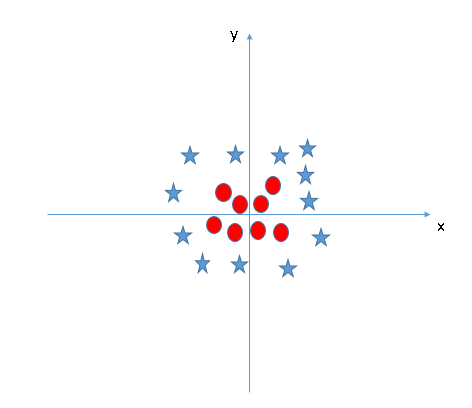
\includegraphics[width=0.4\textwidth]{figure/SVM_non1}
\caption{support vector machine }
\end{figure}

To understand the concept let's map our train data (above figure) to a new feature space $z=x^2+y^2$. Therefore, all values for z would be always positive because z is the squared sum of both x and y as shown by the figure below. So, it is seen from the figure the data can be easily. Therefore, the chance is more for a nonlinear separable data to become linear separable in higher dimensional space.

\begin{figure}[H]
\centering
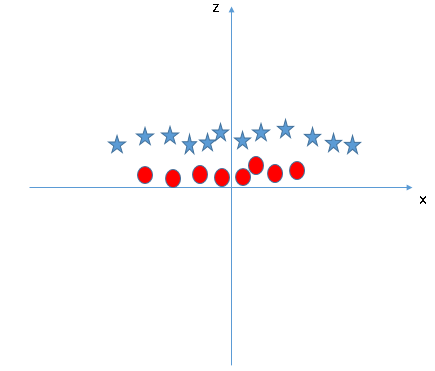
\includegraphics[width=0.4\textwidth]{figure/SVM_non2}
\caption{support vector machine }
\end{figure}
In our original input space the hyperplane should looks like a circle as shown by the following figure.

\begin{figure}[H]
\centering
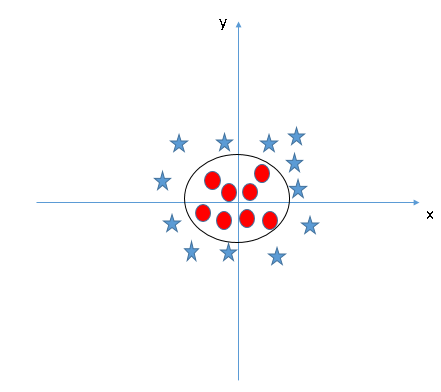
\includegraphics[width=0.4\textwidth]{figure/SVM_non3}
\caption{support vector machine }
\end{figure}

Considering all the concepts above, there still exists the problem of misclassification data. So it is not sufficient just finding decision boundary with maximum margin. Therefore we have to consider the problem of misclassification errors also. So model should be be modified such that it finds the decision boundary with maximum margin but with less misclassification. The minimization criteria is modified like as:

\begin{align*}
\min||\omega||^{2}+C(distance \: of \: misclassified \: samples \: to \: their \: correct \: regions)
\end{align*}
This concept is described by the figure below.
\begin{figure}[H]
\centering
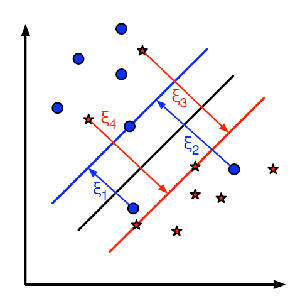
\includegraphics[width=0.4\textwidth]{figure/SVM_non4}
\caption{support vector machine }
\end{figure}
For each sample of the training data a new parameter $\xi_{i}$ is declared. $\xi_{i}$ is the distance from its corresponding training sample to their correct decision region (shown by the read and blue arrows). The samples which are not misclassified and therefore, they fall on their corresponding support planes, their distance is considered as zero.
So the updated optimization problem is:
\begin{align*}
\min_{\omega, b_{0}} L(\omega, b_{0}) = ||\omega||^{2} + C \sum_{i} \xi_{i} \:  \text{subject to} \: y_{i}(\omega^{T} x_{i}+ b_{0}) \geq 1-\xi_{i} \: \text{and} \: \xi_{i}\geq 0 \: \forall i 
\end{align*}
How should the parameter C be chosen, which depends on how the training data is distributed. Although there is no general answer but it is useful to consider the following rules:
\begin{itemize}
\item Large values of C provide solutions with less misclassification errors but a smaller margin. Consider the fact that it is expensive to make misclassification errors. Since the goal of the optimization is to minimize the argument, so few misclassifications errors are allowed.
\item Small values of C provide solutions with bigger margin and more classification errors. In this case the minimization does not consider the summation term of $\xi_{i}$, instead focuses more on finding a hyperplane with big margin.
\end{itemize}
So the choice of the value of parameter C is a trade-off between the misclassifiaction and margin size. 
\section{Random Forest}
Random forest is a supervised learning algorithm and also known as ensemble method. The goal of ensemble method is to build a strong classifier from the the ensemble of several weak classifiers. Decision tree algorithm is used as the weak classifiers. The whole algorithm approaches can be divided as model classifying phase.
\begin{description}[leftmargin=*]
\item[Model Training:]
At first, we create different training datasets, where each dataset holds the same number of samples as the original dataset using Bootstrap method. Bootstrap is the process of drawing sample data as random with replacement. Therefore, some samples will draw more than once and some will be absent. We use these new training datasets for creating the trees. For $N$ numbers of new training datasets, we get $N$ numbers of trees in the forest. At each node of each trained tree, a random subset of the features instead of all features are used to find the best split. With each node a new subset of features is generated and the size of the subset is fixed for all the nodes and all the trees. Generally, If we have $F$ number of features in a sample, then the subset contains $\sqrt{F}$ features. In the forest, none of the built trees are pruned. 
\item [Classifying Phase:] The classifier takes the input sample, classifies it with every tree in the forest and outputs the class label that received the majority of votes. 
\end{description}
The classification phase of the algorithm is shown by the following figure. Where internal or decision node is shown by circle and leaf or terminal node is shown by rectangle.
\begin{figure}[H]
\centering
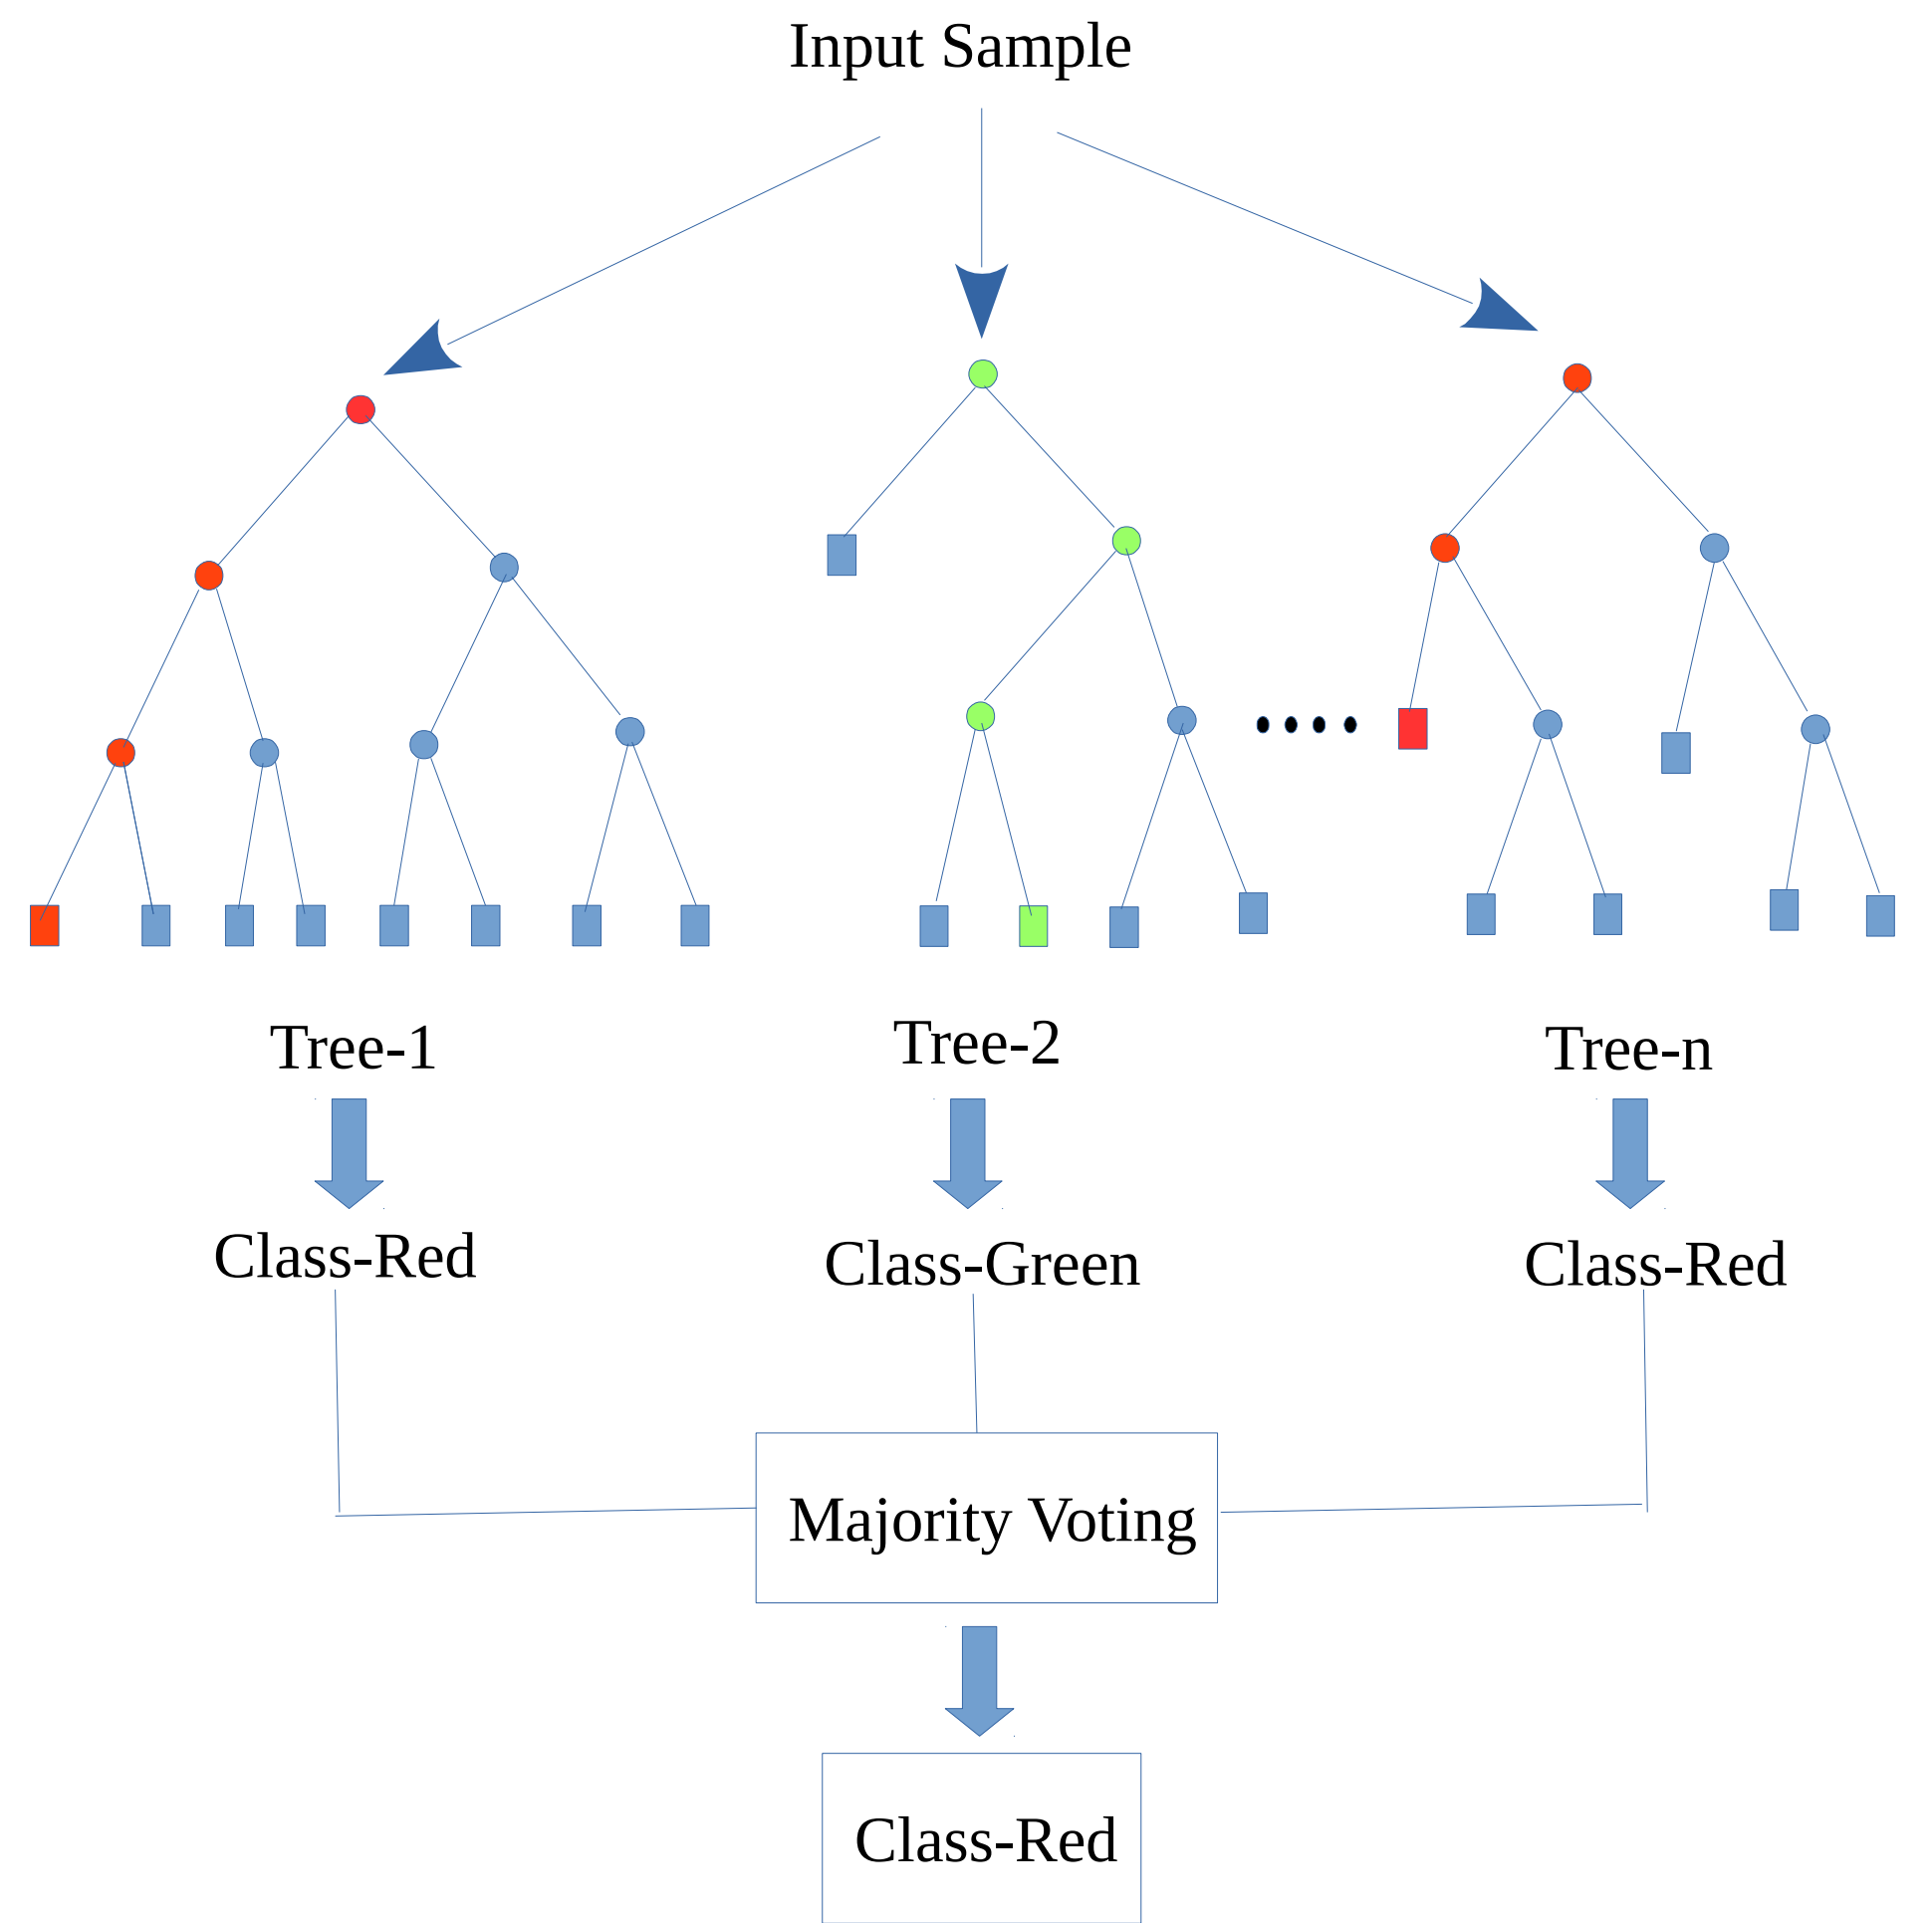
\includegraphics[width=0.8\textwidth]{figure/rf1}
\caption{Random forest Classifier }
\end{figure}

\section{Gradient Boost Tree}
Gradient boosting decision tree(GBDT) is a boosting ensemble algorithm which builds
predictive model by the ensemble of weak models, usually decision trees. GBDT works in
following steps:
\begin{enumerate}
\item Optimization of a loss function.
\item Predictions by a weak model.
\item Adding weak model to minimize loss function.
\end{enumerate}
The pseudo code of boosting algorithm is given below:
The input training set ${( x_{i} , y_{i} )}_{i=1}^{n}  $ and for $M$ number of iterations, the loss function is $L ( y, f ( x ))$
\\1.Initialize weak model which can be written as:
\begin{align}
 F_{0} ( x ) = \underset{\gamma}{\mathrm{argmin}} \sum_{i=1}^{n} L ( y_{i} , \gamma )
\end{align}
2. For $M = 1$ to $m$, compute the gradient as:
\begin{align}
z_{im}=-[\fdv{L(y_{i},f(x_{i}))}{f(x_{i})}]_{f=f_{m-1}}
\end{align}
where $i = 1,.....,n$
\\
3. Fit base tree $g_{m}(x)$ to predict the targets $Z_{im}$ for all training data.
\\
4. Compute gradient descent step size as:
\begin{align}
 \gamma_{m} = \underset{\gamma}{\mathrm{argmin}} \sum_{i=1}^{n} L ( y_{i} , f_{m-1}(x_{i})+\gamma g_{m}(x_{i}) )
\end{align}
\\
5. Update the model as :
\begin{align}
 f_{m}(x)=f_{m-1}(x)+\gamma g_{m}(x))
\end{align}
6. Return the final model $ f_{M}(x) $
ensemble.GradientBoostingClassifier and ensemble.GradientBoostingRegressor pack-
ages are implemented GBDT for classification and regression algorithm, respectively.
\section{K-Nearest Neighbor}
K-nearest neighbor (KNN) is very simple but powerful supervised learning algorithm, which is used both for classification and regression problems. The algorithm works in three steps.

\begin{itemize}
\item Firstly, for given a positive integer $K$ and a test sample $x_{0}$, the KNN classifier recognizes the neighbors K points in the training data that are closest to $x_{0}$, denoted by $N_{0}$.
\item Secondly, It calculates the conditional probability for class $j$ as the fraction of
points in $N_{0}$ whose response values are equal to $j$. The conditional probability is given by the following equation \cite{james2013introduction}:
\begin{align}
P_{r}(Y=j|X=x_{0})=\dfrac{1}{K} \sum_{i \in N_{0} } I(y_{i}=j)
\end{align}
Where, $I(x_{0})$ is the indicator function which evaluates to 1 when the argument $x_{0}$ is true and 0 otherwise.
\item Finally, KNN classifies the test sample $x_{0}$ to the class with the largest probability.
\end{itemize} 
Now we illustrate how KNN algorithm works with the following figure. We have plotted a small training data set consisting of five red stars and eight green circles observations. Let's say stars and circles are in red and blue classes respectively. Our aim is to make a prediction for the test data labeled by the blue rectangle.

\begin{figure}[H]
\centering
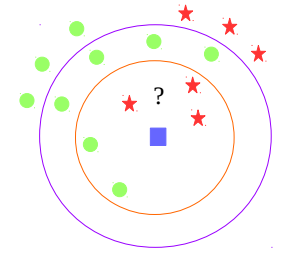
\includegraphics[width=0.3\textwidth]{figure/KNN3}
\caption{Simple figure to explain KNN algorithm}
\end{figure}
 
In the first case, suppose that we choose $K = 5$. Then KNN will first recognize the five observations that are closest to the blue rectangle. This neighborhood is shown as a circle of orange color. It consists of two green points and three red points. So the resulting estimated probabilities for the red class is 3/5 and for the green class is 2/5. Hence KNN will predict that the blue rectangle belongs to the red class.
\\\\ In the second case, assume that we choose $K = 9$. Then algorithm first identifies the nine observations that are closest to the blue rectangle. This time neighborhood is displayed as a circle of purple color. It has six green points and three 3 red points. Therefore, the resulting estimated probabilities for the red class is 3/5 and for the green class is 6/5. Hence KNN will predict that the blue rectangle belongs to the green class. To avoid the tie condition, the value of $K$ should be chosen as odd integer number.

\chapter{Dataset and Evaluation Method}
\section{Result Evaluation Terms}
\subsection{Classification evaluation method}
\textbf{Confusion matrix:}
A confusion matrix has information about actual and predicted class labels done by a
model. The data in the matrix are commonly used to evaluate performance of such model.
The following table illustrates the confusion matrix for binomial classification model.
\begin{center}
\begin{table}[h]
\begin{center}
\caption{\label{tab:table-name}Confusion Matrix}
\begin{tabular}{|l|l|l|l|}
\hline
\multicolumn{2}{|l|}{}                                                      & \multicolumn{2}{c|}{\textbf{Predicted}}                 \\ \cline{3-4} 
\multicolumn{2}{|l|}{\multirow{-2}{*}{}}                                    & \textit{Positive}          & \textit{Negative}          \\ \hline
\multicolumn{1}{|c|}{}                                  & \textit{Positive} & \cellcolor[HTML]{67FD9A}TP & \cellcolor[HTML]{FFCE93}FN \\ \cline{2-4} 
\multicolumn{1}{|c|}{\multirow{-2}{*}{\textbf{Actual}}} & \textit{Negative} & \cellcolor[HTML]{FFCE93}FP & \cellcolor[HTML]{67FD9A}TN \\ \hline
\end{tabular}
\end{center}
\end{table}
\end{center}
The data in the confusion matrix has the following meaning:\\
TP is the number of true predictions that an instance is positive,\\
TN is the number of true predictions that an instance is negative,\\
FP is the number of false predictions that an instance is positive,and\\
FN is the number of false of predictions that an instance negative.\\

\textbf{Accuracy Score:}
Accuracy score is the most common evaluation metric for classification models. It is the
number of correct predictions as a ratio of the total number of predictions. The best
accuracy is 1 and the worst is 0.0. It can be calculated as:
\begin{align}
Accuracy = \dfrac{\sum TP+ \sum TN}{\sum TP + \sum T N + \sum F N + \sum FP}
\end{align}


\textbf{Recall:}
Recall is the number of correct predictions as a ratio of the total number of positives. It
is also call the true positive rate. It can be written as:
\begin{align}
Accuracy = \dfrac{\sum TP}{\sum TP + \sum FN}
\end{align}

\textbf{Precision:}
Precision is the number of correct positive predictions as a ratio of the total number of
positive predictions. It can be written as:
\begin{align}
Accuracy = \dfrac{\sum TP}{\sum TP + \sum FP}
\end{align}

\textbf{ROC Curve:}
ROC curve illustrates relative tradeoffs between true positives and false positives. It is atwo dimensional graph in which recall is plotted on the Y axis and specificity is plotted on the X axis.Specificity is the number of correct negative predictions as a ratio of the total number of negative predictions.A binomial model is one that outputs only a label.Figure shows binomial models. Some points are important in ROC space. The lower left point (0,0) depicts the strategy of never issuing a positive classification; such a model does have no false positive errors but also no true positives gain. The point (0, 1) means this is a
perfect classification such as performance of D's.In contrast, the performance of E's is
worst.
\begin{figure}[H]
\centering
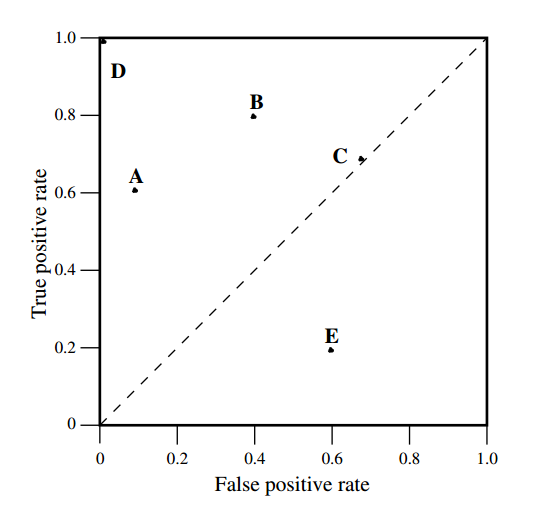
\includegraphics[width=0.7\textwidth]{figure/roc_1}
\caption{A basic ROC graph showing five discrete classifiers.}
\end{figure}

\subsection{Cross Validation}
Cross validation is a method for evaluating predictive models. It is better than residuals.
There is no indication about how well the model will predict for new unseen data in
residuals.This problem can be overcome by not using entire data set when training a
model. A portion of data is removed before training the model. This removed data will
be used for testing the model performance on new data. This idea is cross validation.
holdout method and k-fold cross validation methods are used to evaluate the model
performance of this study.
Holdout Method:
It is the simplest type of cross validation. The data set is splitted into two sets as training
sets and testing set. The model is trained with the training set and then testing data used
for prediction. As the splitting training and testing sets are independent, the evaluation
result may be different.
K-fold cross validation:
In K-fold cross validation, the data set is split into k subsets. Each time k-1 subsets
are put together and sued to train the model, and rest one subset used to evaluate the
model which was not used to train. This process is repeated for k times where each time
different subset used for evaluation. Then the average error across all repetitions is
computed. It can detect the overfitting. Each data point is tested. The computational

\begin{figure}[H]
\centering
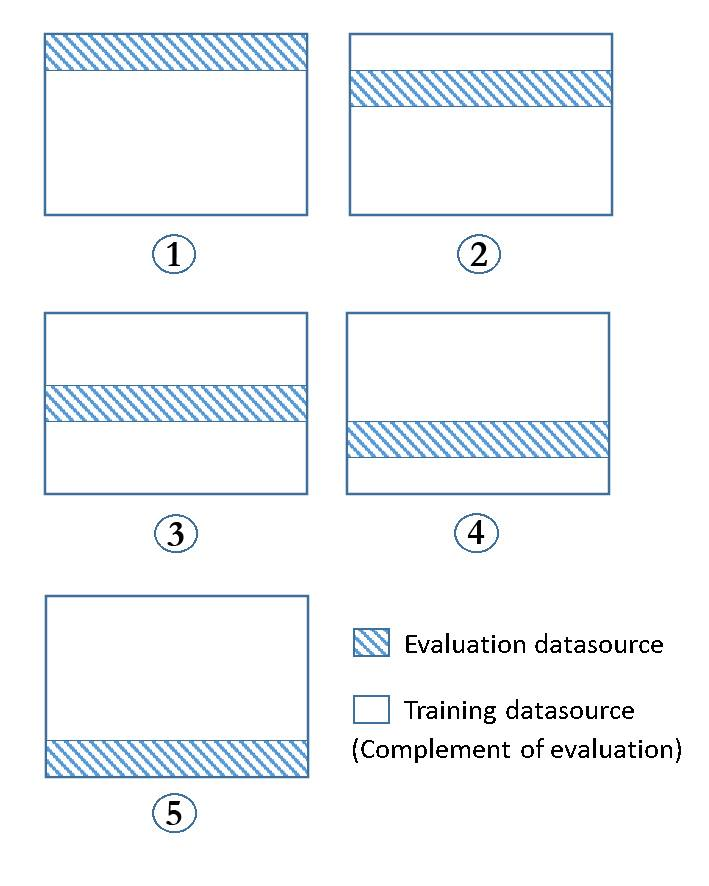
\includegraphics[width=0.5\textwidth]{figure/cros}
\caption{Splitting dataset in 5-fold cross validation. Reproduced from}
\end{figure}
time is high compared to holdout method. It is possible to choose independently how
large the each test set. The Figure 6.2 shows an example of k-fold cross validation where
k = 5. First 20 percent of data used for evaluation and rest 80 percent for training in
model one. Second 20 percent (21-40 percent) used for evaluation and rest subsets for
training and so on.
To evaluate predictive models of this study, k=10 is used for cross validation. 10-
fold cross validation is used only for regression models where the dataset has 147473
observations.

\chapter{System Overview}
From the recent past till now a lots of researches has been going on in the field of robotics, specially how to equipped a robot with perceptual capabilities. Therefore, a new brunch of robotics has been immersed is known as cognitive robotics or robotic perception, where people research how to build an intelligent robot or machine. To get human like perception from a robot is still a dream. There is huge gap between the functionalities require for a robot performing human-scale manipulation tasks and the functionalities today's perception algorithms provide with. However there are some robots in the lab environment, which already equipped with some perceptual capabilities. It is easy task for a human to recognize a object from a table. But for the same task, a robot needs a lots of complicated approaches and perception algorithms.
\\\\The field of image processing and robotics are complementary with each other. In the history of image processing, there were huge numbers of researches have been carried out and a lots of algorithms has been developed. People preserved these research works as programming library and framework, so that the research work can be used later. There are quite significant numbers of libraries exist, which provide the perception algorithms.
\\\\ In the aim to facilitate and organize the research work in the field of robotic perception, the institute for artificial intelligence developed a perception framework called \textbf{roboSherlock} \cite{beetz2015robosherlock}. The framework has been designed to work with perception algorithms that exist in different libraries and provides a common place to integrate these algorithms flexibly. Since, our developed perception system for this thesis work is based on \textbf{Robosherlock}, so at first we will give an overview of the components and functionalities of \textbf{roboSherlock} in the following section. After that we will illustrate about our implemented system and it's usages.


\section{RoboSherlock}
Robosherlock is based on the open source framework UIMA (Unstructure information management architechture). UIMA is a software framework for the analysis of unstructured data such as text documents, video or audio data. It is a pluggable architecture allowing integration and modularization, and has been proven to be a powerful tool for unstructured information processing.Perhaps the most famous example of a UIM system is Watson \cite{ferrucci2010building}, a question answering system that competed against the champions of the quiz show called jeopardy and and won the quiz show. In UIM, pieces of unstructured informations are processed by a collection of specialized information extraction algorithms (called annotators) and each algorithm contributes pieces of knowledge with respect to their expertise. Therefore, the output knowledge collected from different annotators are combined to get the consistent final decision. The infrastructures and components of the UIMA is shown by the following figure.
\begin{figure}[H]
\centering
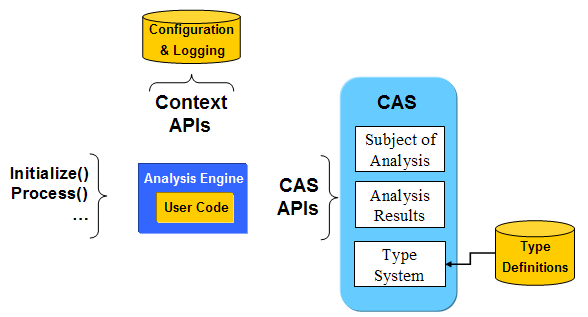
\includegraphics[width=0.7\textwidth]{figure/framework}
\caption{UIMA Framework Core}
\end{figure}
RoboSherlock inherits the basic data structure and components of control mechanism from UIMA. As mentioned in \cite{balint2017storing} a user defined type system serves as a blue-print for the internal data structure and permits communication between the components of the framework through the common analysis structure (CAS). The CAS acts as a white-boards architecture, allowing components to post and retrieve data solely based on the type system. At any given times, components only need to know only the data types they are supposed to post or send to CAS. The main components of the framework is Analysis engine.
there are two types of analysis engines depending on functionality. The first one is primitive analysis engine (Annotator), which is used to provide the functionality of a single method or algorithm. The second one is aggregate analysis engine (ensembles of annotators), which provides the complete functionalities of a perception system. It is also known as the pipeline. The annotators are mainly perception algorithms from libraries OpenCV (open source computer vision) and PCL (Point Cloud Library). The complete work flow of a pipe line are describe using the following figure. 
\begin{figure}[H]
\centering
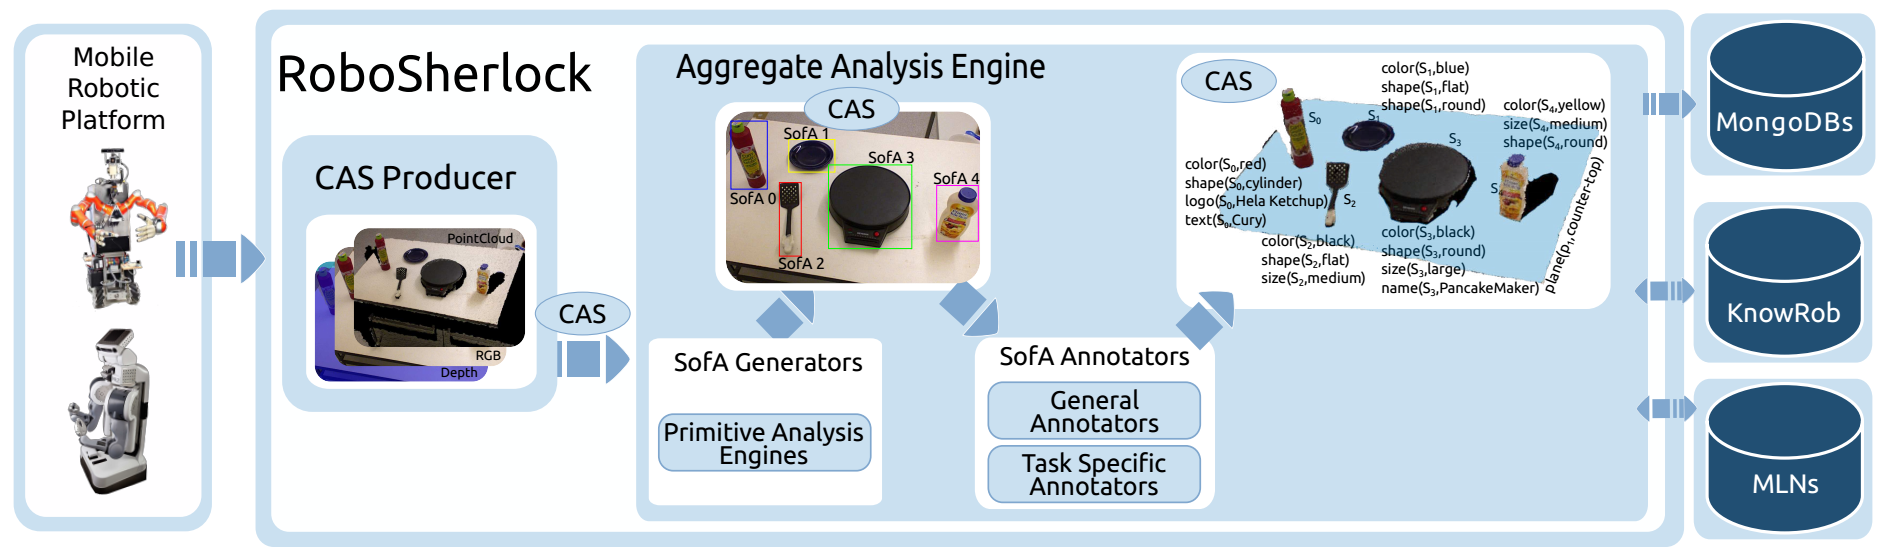
\includegraphics[width=0.9\textwidth]{figure/roboPipe}
\caption{Example of pipeline execution in Robosherlock}
\end{figure}
The sensor data used by the pipeline is generated by a Kinect camera mounted on the head of the robot. The data is typically standard RGB color image and point cloud (depth-RGB image), which is a set of 3D point in space represents the external surface of an object.
Robosherlock considers row sensor data (image scene) as unstructured information in which it tries to find pieces of data that represent object or object groups. These pieces of data is called hypothesis or Sofa (subject of analysis), which are produced by annotators, consist of image segmentation and clustering algorithms. After that the hypotheses are annotated with symbolic (e.g. class label) or sub-symbolic (e.g. color histogram) information. Depending on the task at hand, the annotations are used to test and rank the possible answer. In the pipeline the output of one annotator can be the input of another annotator. If someone wants to store the data precessed by pipeline for further analysis, there is a storage writer annotator, which writes data in database.The database is consider as the memory of robosherlock. The storage writer annotator should placed at the end of the pipeline. When the pipeline processing is finished, the CAS gets reset and new processing loop starts again.
\subsection{Memory For Robosherlock} 
In cognitive psychology, memories are categorized into short-term and long-term memory, where the short-term is a small capacity storage that provides the context for executing the current task. The long-term memory is a high volume memory that gives comprehensive information for all sorts of tasks and \cite{wood2012review} can be further categorized as procedural or declarative memories. Declarative memory is often considered as consciously accessible and the procedural memory consists of compiled or subconscious information. Episodic memories store experienced event information that is temporally and spatially organized and combined with context information. Episodic memories has great importance in robotic perception \cite{}, because they enable robots to "relive" past events and learn from them. 
\\\\ The framework provides MongoDB database based state of the art memory system for robotic agents performing manipulation tasks in kitchen environment \cite{balint2017storing}. The reason of choosing MongoDB as the storage location because it is a schema-less database means it doesn't have any fixed data structure. This property nicely matches the paradigms of unstructured information processing, as nobody can not ensure that ever hypothesis will be annotated in the same way or that every execution loop produces the same views. MongoDB organizes data in collection and documents. The top level structure of the collections of the database and their relations are shown by the following figure. 
\begin{figure}[H]
\centering
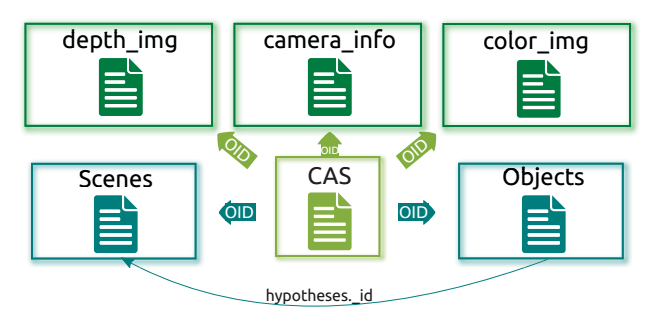
\includegraphics[width=0.9\textwidth]{figure/database_top}
\caption{Top level structure of MongoDB and relation bewteen collections taken from \cite{Storing}.}
\end{figure}
 The collections are connected with each other by unique Id (OID). They are indexed on the timestamps of the incoming data and  previously mentioned unique ids are automatically generated by the MongoDB client. Inside collections documents are arranged as key pair value structure. As the names of the collections in the top row infer that they contain information about  the point cloud (Depth image), camera and color image receptively. 
\\\\ The CAS collections contains the OID (ObjectId) of the documents all other collections and acts as a parents. One can programmatically manage the "ObjectId" of a documents from CAS and can access documents correspond with this "ObjectId" from all other collections. The CAS collection for a single document is shown as follows.   
\begin{figure}[H]
\centering
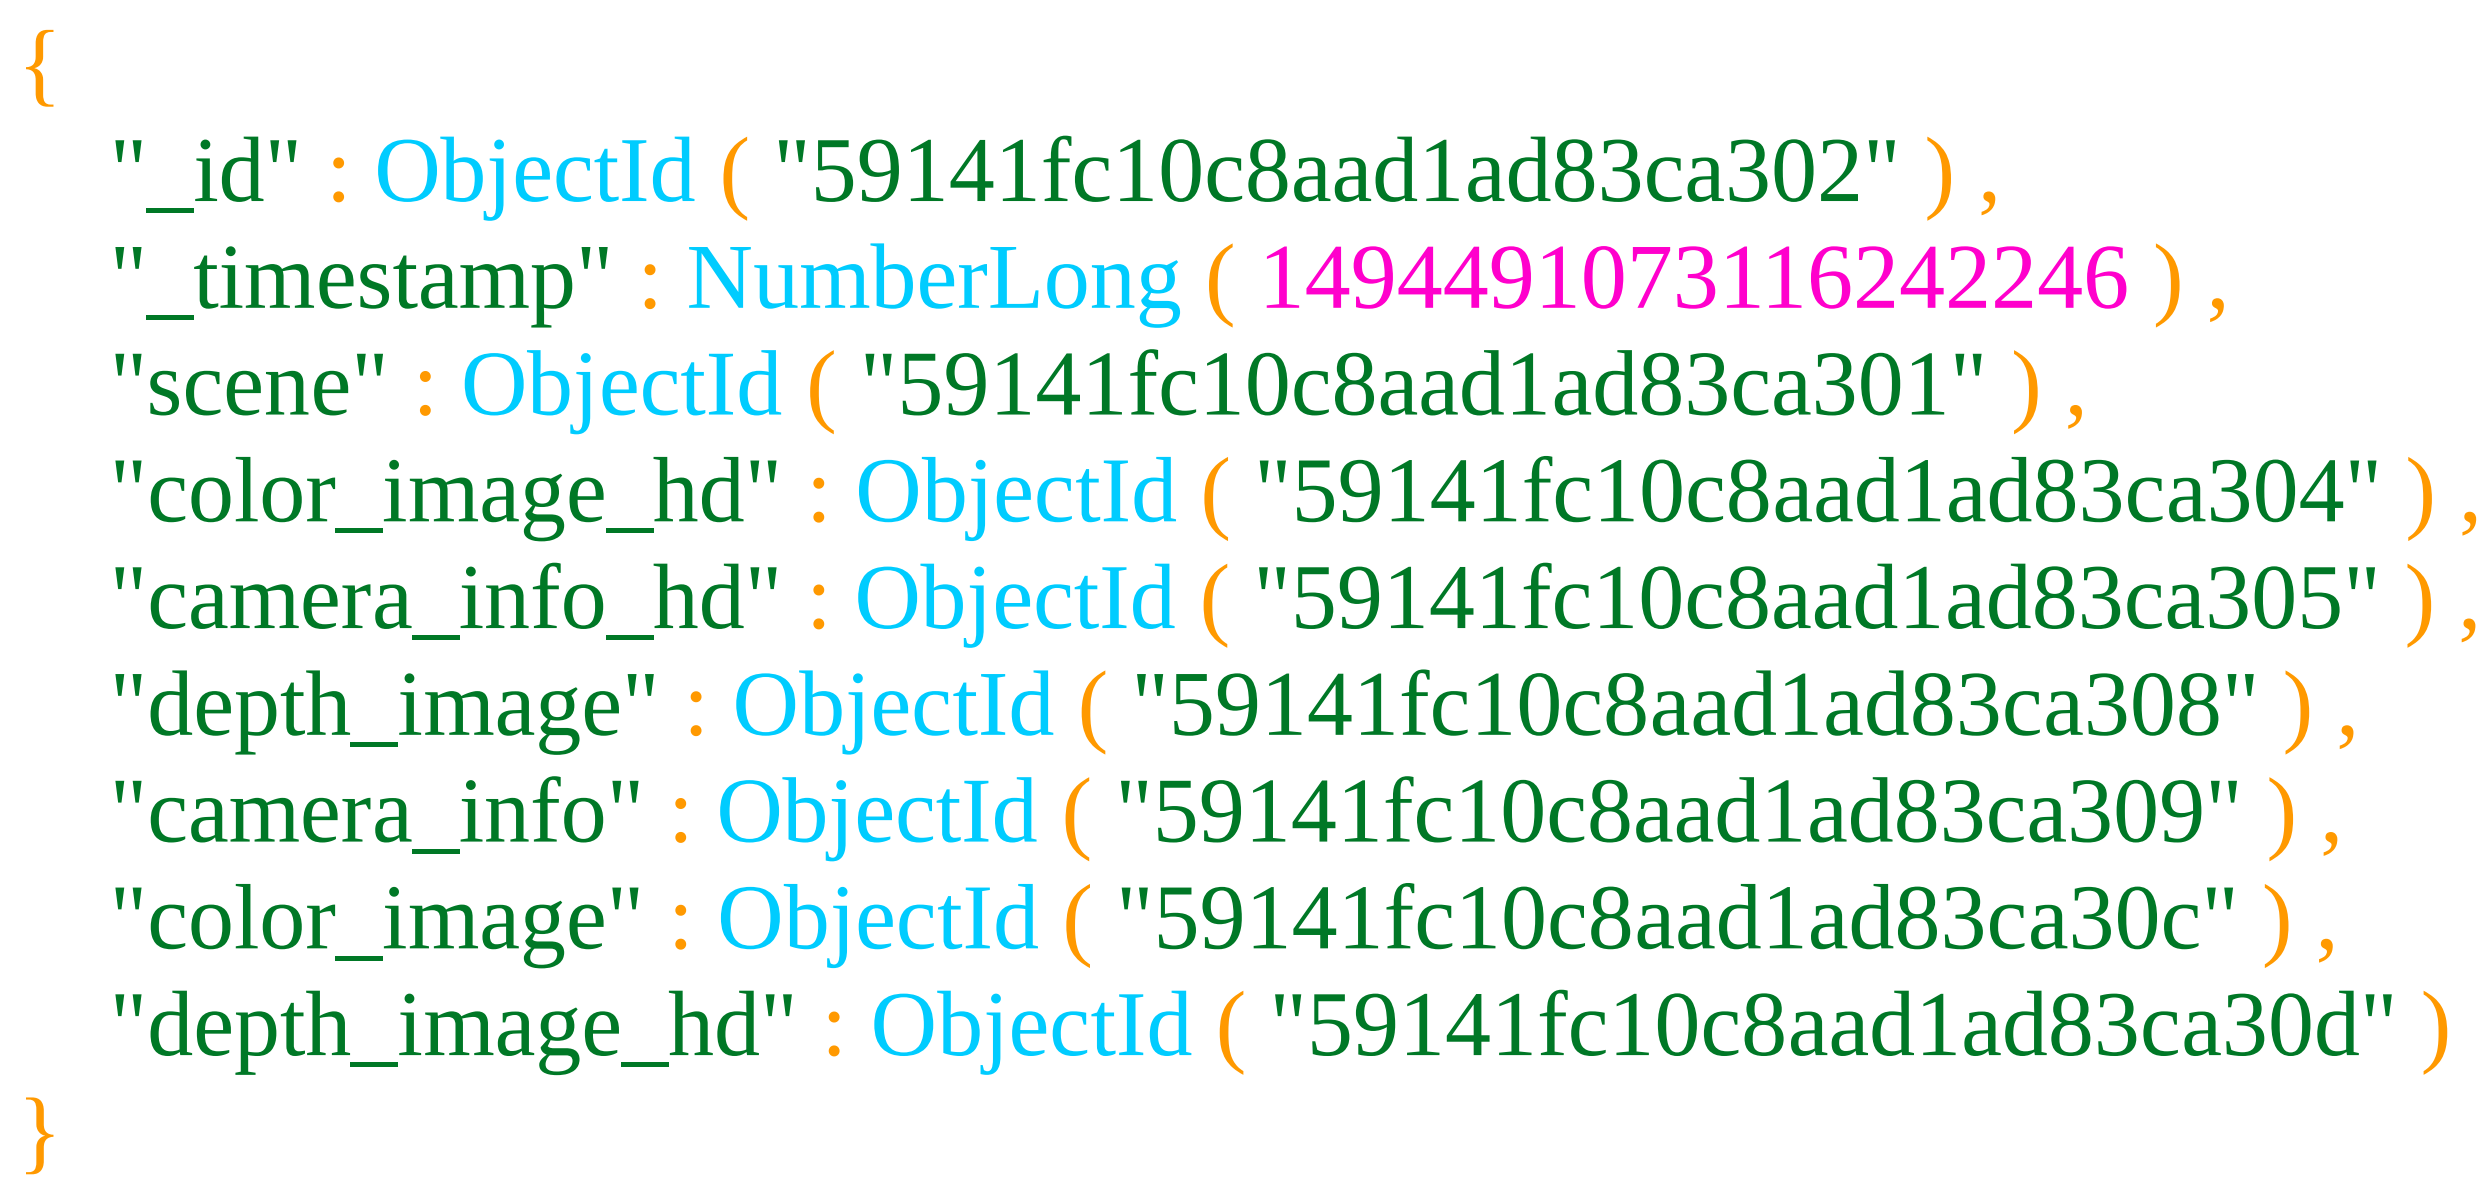
\includegraphics[width=0.9\textwidth]{figure/cas1}
\caption{The cas collection}
\end{figure}
Every perception system that runs during long-term task, needs to build a belief state about the world. The "objects" collection contains the objects that are believe to be exist in the environment after entity resolution and are connected to the individual instances through the IDs of the object hypotheses that are located in scenes collections as mentioned in \cite{balint2017storing}. 

\begin{figure}[H]
\centering
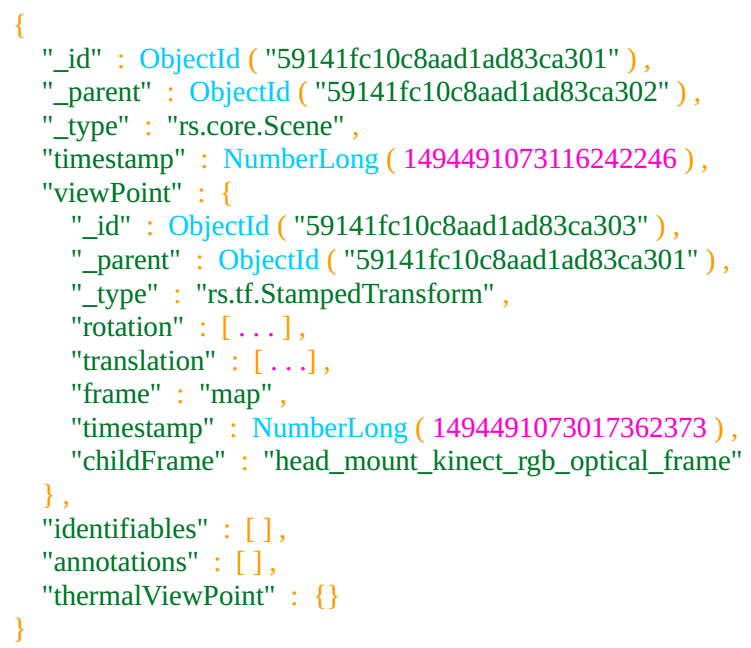
\includegraphics[width=0.7\textwidth]{figure/scene1}
\caption{The scene collection}
\end{figure}

\begin{figure}[H]
\centering
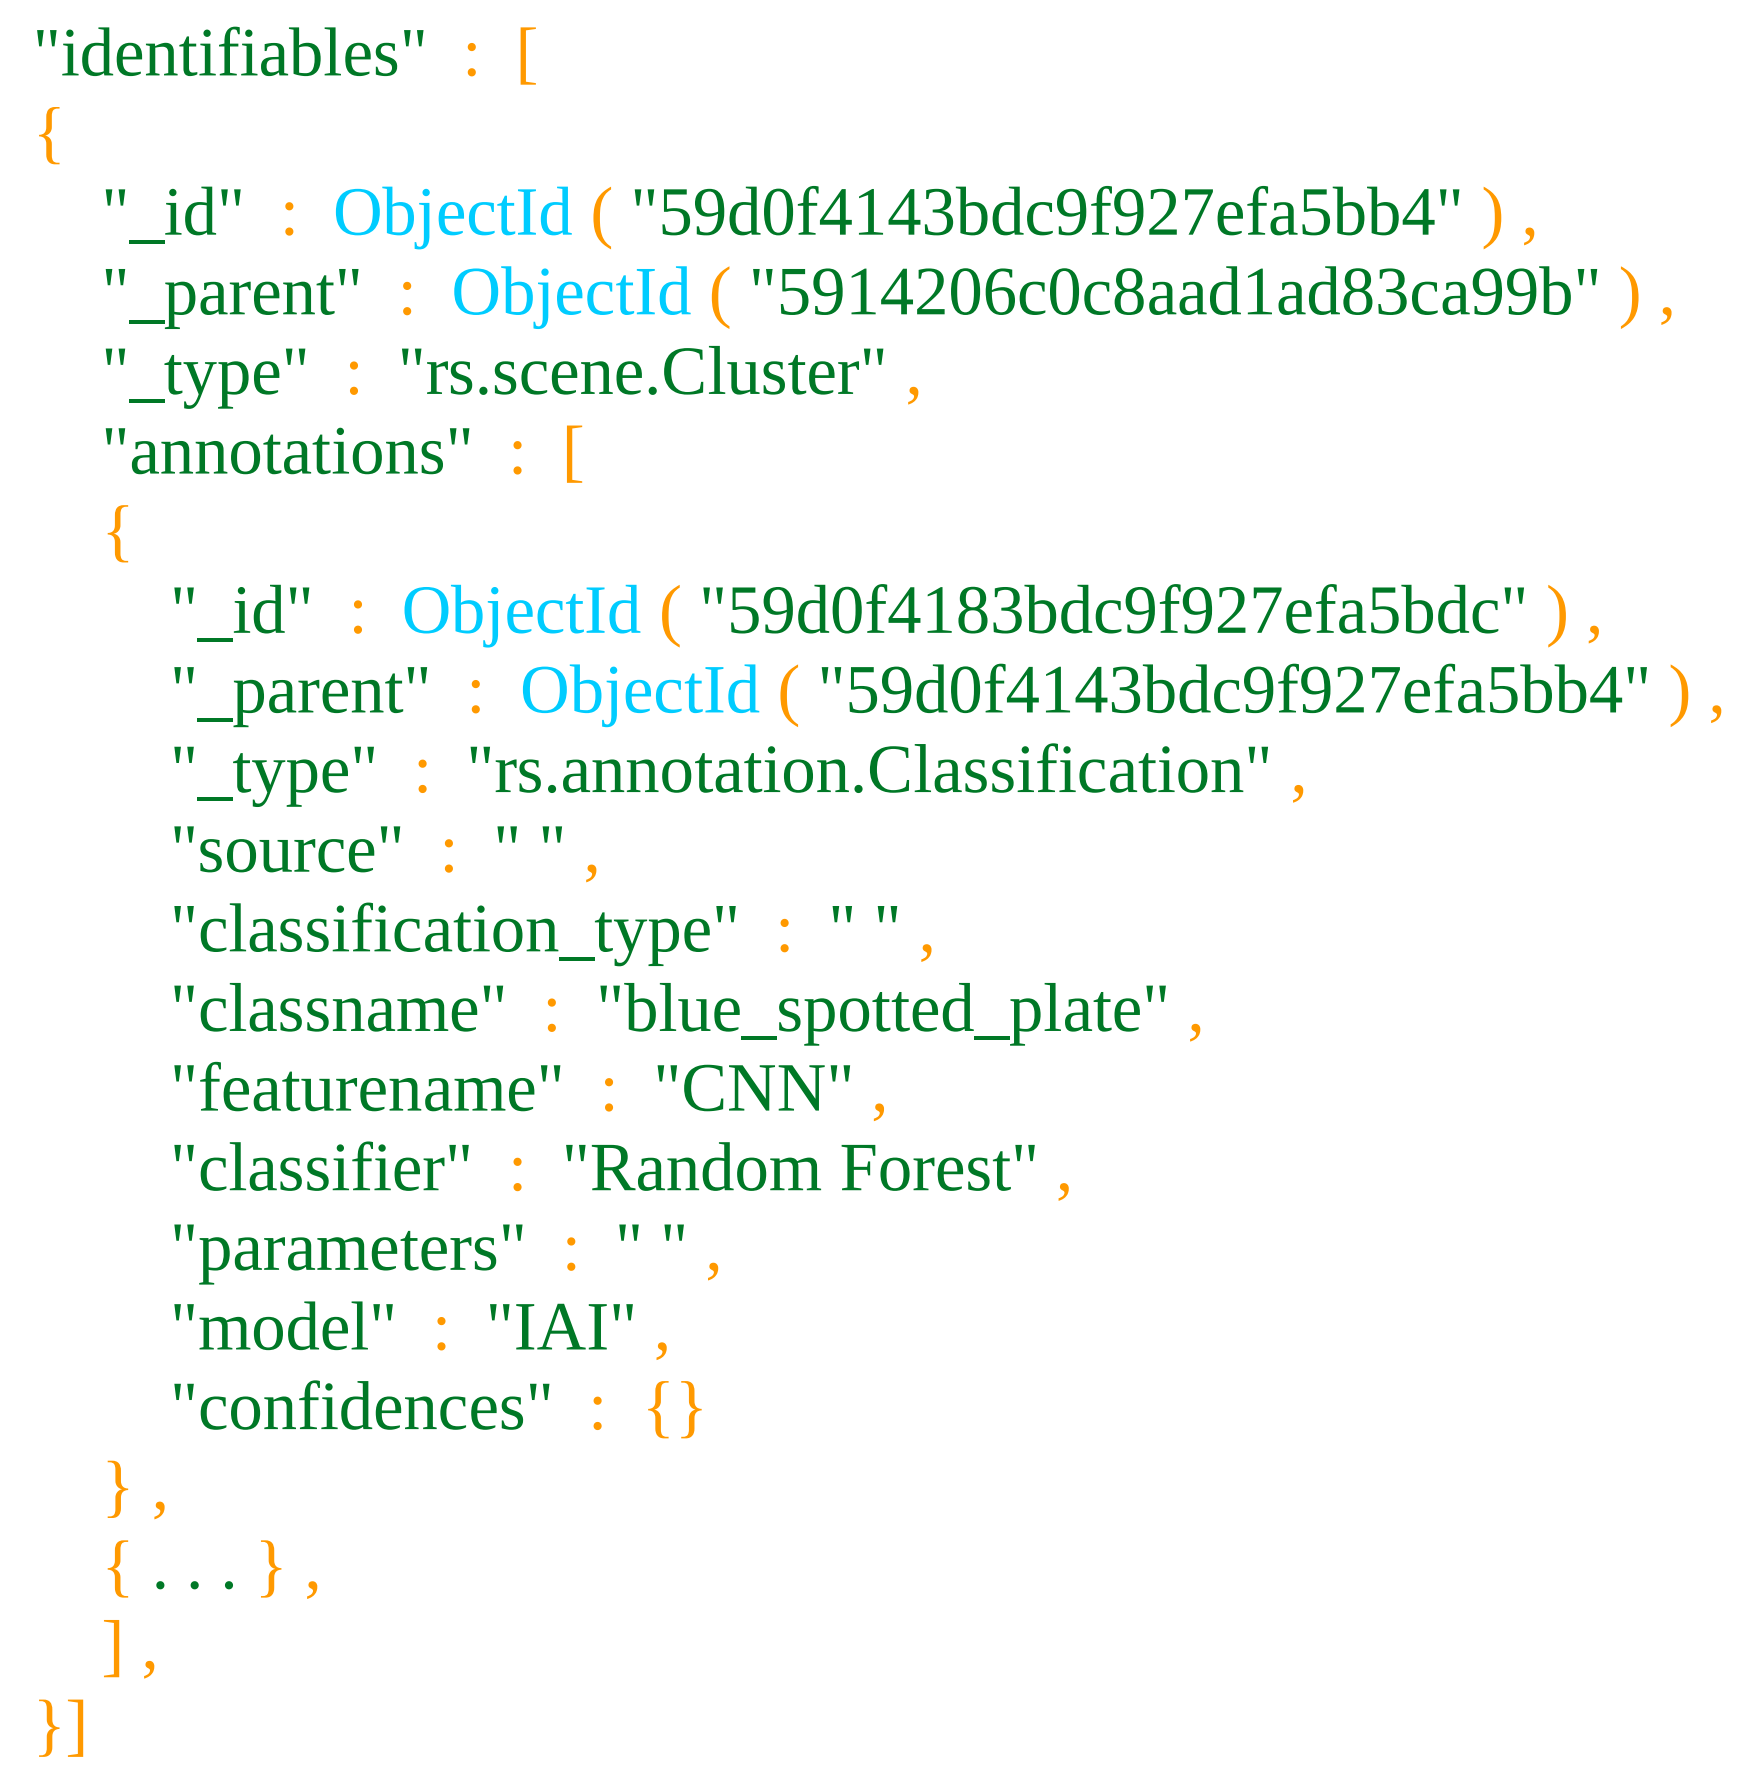
\includegraphics[width=0.7\textwidth]{figure/identifiables1}
\caption{Structure of identifiables in a scene document }
\end{figure}



\begin{figure}[H]
\centering
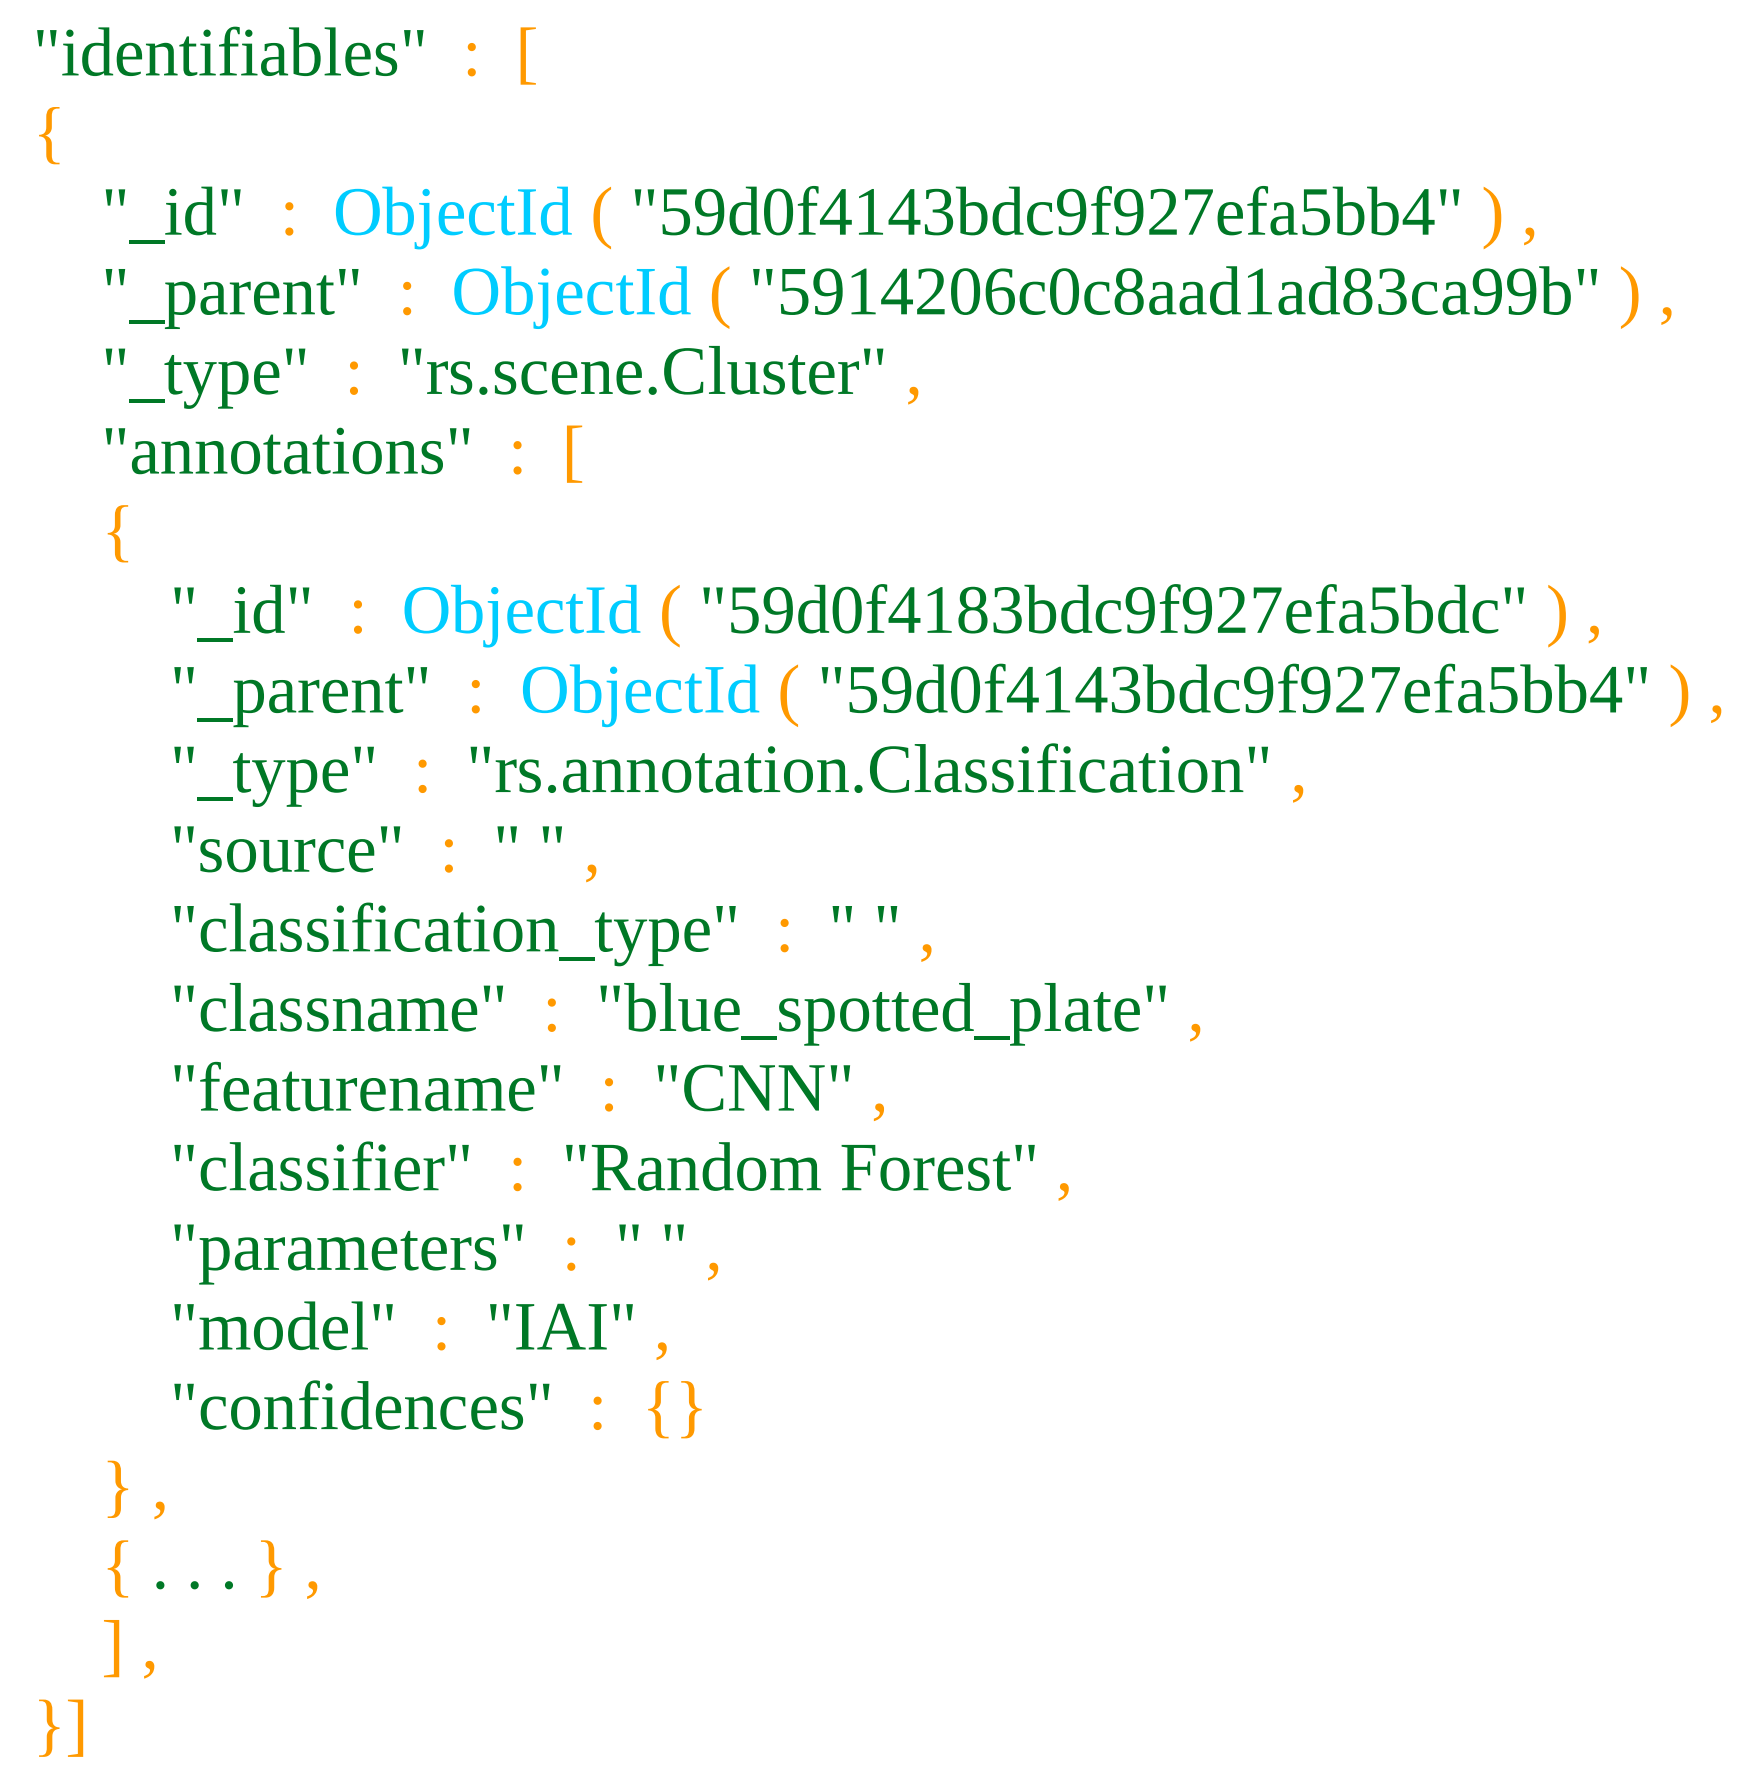
\includegraphics[width=0.7\textwidth]{figure/identifiables1}
\caption{Structure of identifiables in a scene document }
\end{figure}

\subsection{Web based Visualization tools}
As the database contains the meta information, so it is not understandable which annotations are wrong. The frame work also provides a javascript based visualization tools \cite{Storing}. It helps researcher to understand when the robot makes mistakes during the manipulation tasks. So he takes right measures from the errors.

\begin{figure}[H]
\centering
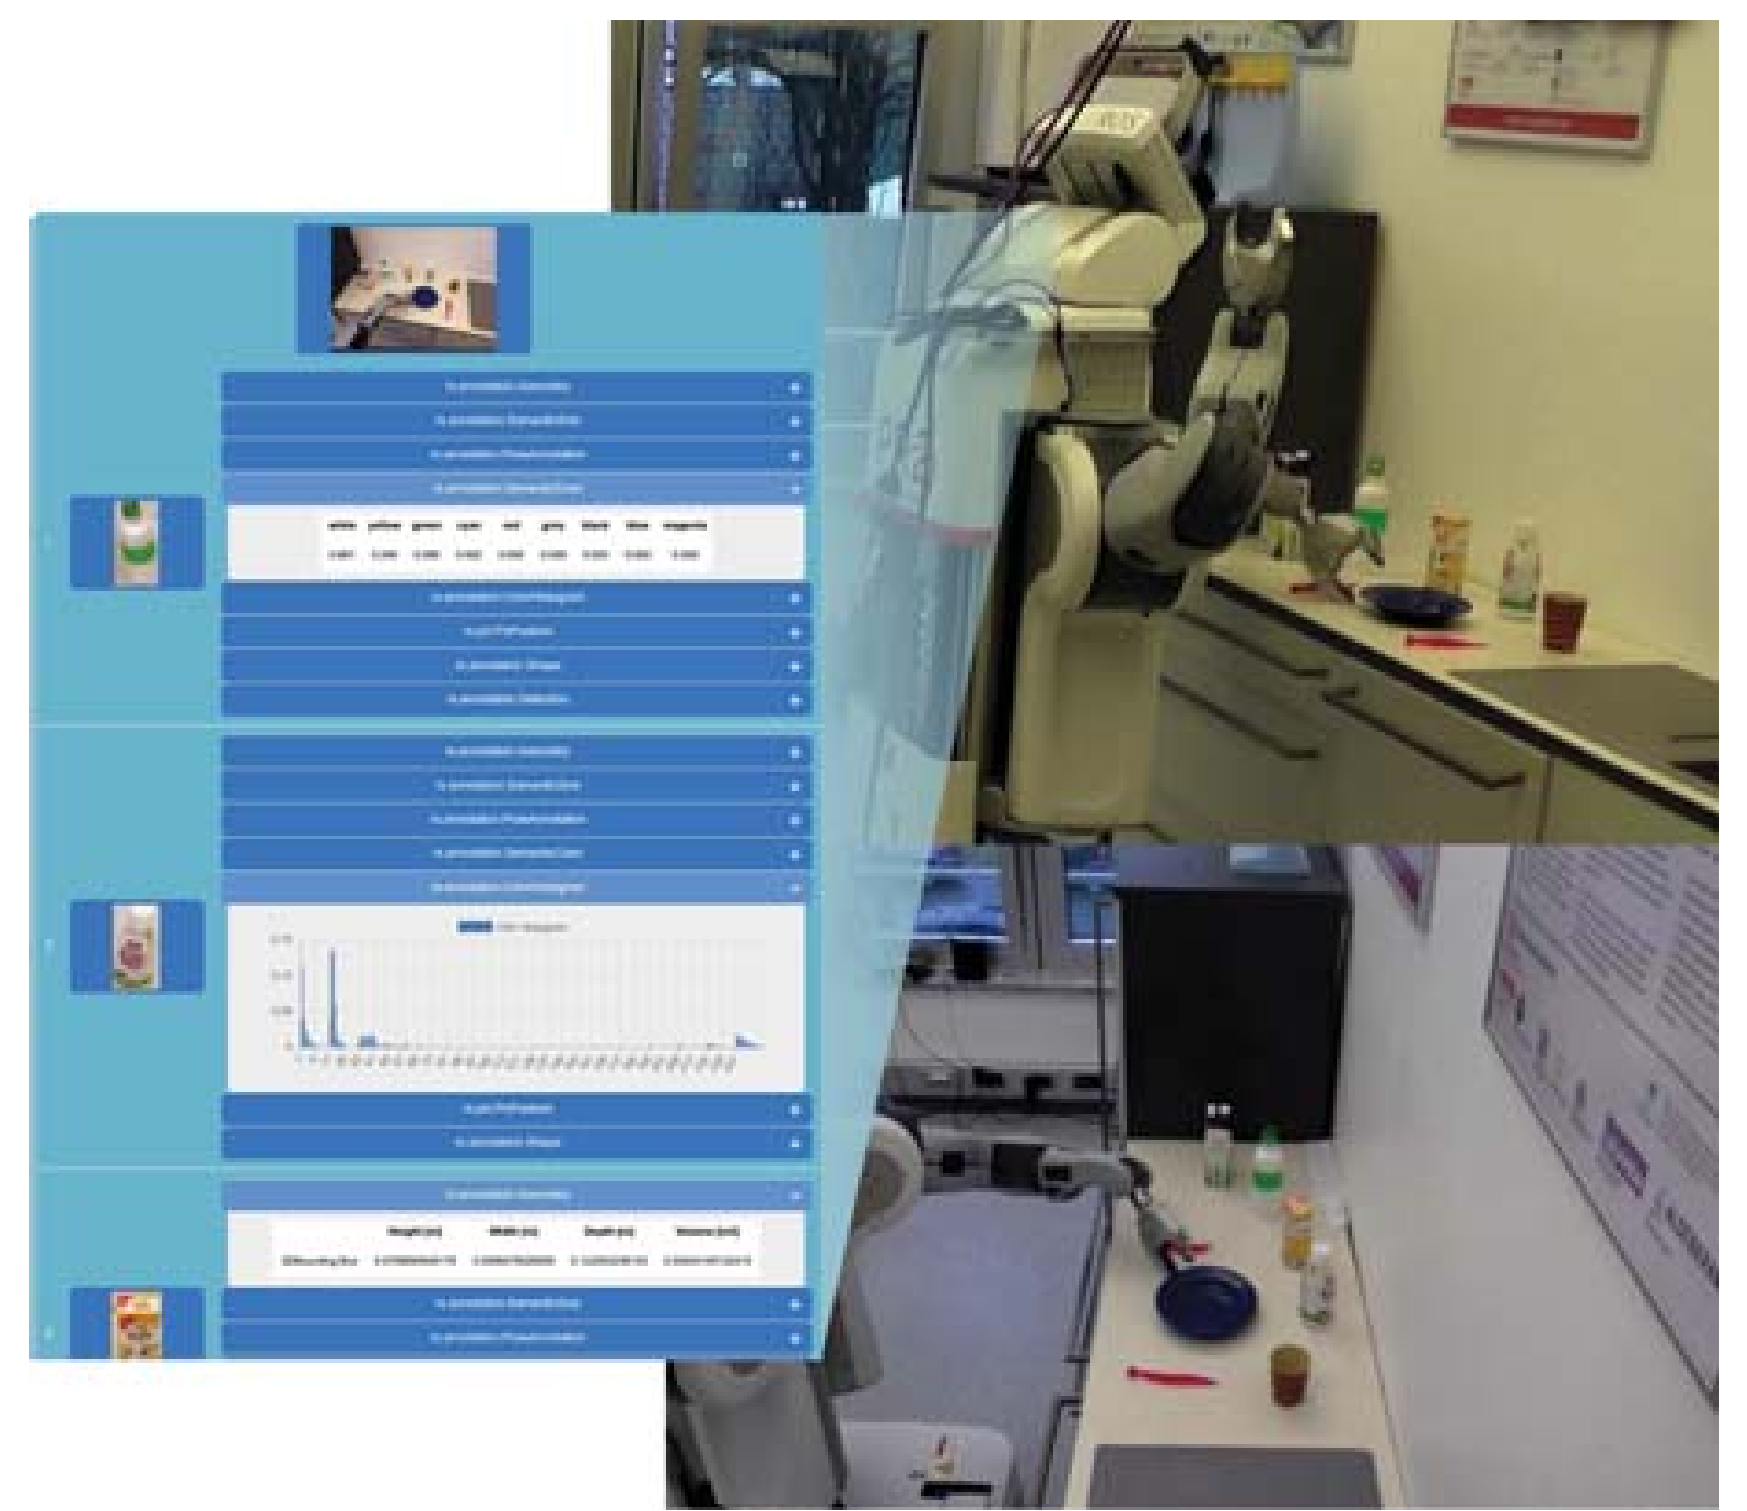
\includegraphics[width=0.7\textwidth]{figure/website}
\caption{Structure of identifiables in a scene document }
\end{figure}
\newpage
\section{Developed System's Architecture}
To implement this thesis work, we had to exploit quite significant number of tools or software code. This tools are mostly wrapped with different perception and machine learning algorithms from different perception frameworks or libraries. We consider
\textbf{Robosherlock} is our main target framework to implement our work. Some of the tools are already existed in the framework and we also developed some tools on top \textbf{Robosherlock} using other libraries. As the \textbf{Robosherlock} is build by \textbf{C++} programming language, so we use the same language for developing tools, which are utilized to work together with all ready existed one. We use \textbf{python} programing language to work with the episodic memory and to evaluate different experiments, which we have done through the entire thesis work. We use web based python library called \textbf{flask} and the markup language \textbf{HTML} to add the ground truth annotation tool on top of already existed web based visualization tool and also add some extra functionalities to visualize the ground truth information of the object hypotheses. The usages of the implemented tools are given in index. The overview of the developed tools and their functionalities are described by the consecutive flow diagrams are given below. These flow diagrams also resemble the works flows of this thesis.   

\subsection{Work Flows from extracting feature to predictive model evaluation:}
As we already mentioned, in this thesis work we focus on supervised learning algorithms for the classification tasks. For the supervised learning problem we need data with ground truth, which is actually the object name or class label. The \textbf{FeaturExtractor} tool takes input as the dataset, extracts features from every image and set a label for the corresponding object in the image. After that, it splits the dataset as training and test data, where every forth image in the dataset considers as test data and rest of the data is used to train the classifier. Therefore, we get approximately $75\%$ as training data and $25\%$ as the test date, which is used for the cross-validation of the predictive model. The \textbf{FeaturExtractor} tool is wrapped with feature extraction algorithms from \textbf{PCL} and deep learning framework called \textbf{Caffe} through \textbf{openCV} library. The algorithms are VFH, CVFH and CNN which is trained on two different networks called BVLC{\_}CFC7 and VGG16. The algorithms have been already illustrated in chapter 2. The usages of the tool are given in index A.1.  
\\\\In the first step, we train the specific classifier using \textbf{ModelTrainer} tool. The tool takes training data as input and generate the predictive model of the specific classifier. The tool is wrapped with popular machine learning algorithms like random forest, support vector machine, K-nearest neighbor and gradient boost trees from \textbf{openCV} machine learning module. The usages of the tool is given in index.A.2.
\\\\After that, we evaluate the performance of the trained or predictive model using \textbf{ModelEvaluator} tool. The tool takes inputs as the predictive model and the test data generated during the feature extraction step. As output it generates the confusion matrix, which describe the classification results of the test data and the overall accuracy of the classifier. The usages of the tool are illustrated in index.A.3. The whole processes are shown by the following flow diagram.

\subsubsection*{Flow Diagram}
\begin{figure}[H]
\center
\tikzstyle{background}=[draw,rectangle,rounded corners,fill=red!50,text width=4em,text centered,minimum height=6mm]
\tikzstyle{block}=[draw, fill=blue!20, rectangle, minimum height=3em, minimum width=6em]
\tikzstyle{blockTool}=[draw, fill=green!20, rectangle, minimum height=3em, minimum width=6em]
\tikzstyle{anblock}=[draw,rectangle,fill=pink!50,text width=15em,text centered,minimum height=6mm]
\tikzstyle{preparation}=[draw,chamfered rectangle,chamfered rectangle xsep=2cm,fill=blue!50]
\tikzstyle{sub}=[draw,rectangle split,rectangle split horizontal,rectangle split parts=3,minimum height=6mm,fill=pink!50]
\tikzstyle{decision}=[diamond,draw,fill=green!50]
\tikzstyle{line}=[draw,-stealth,thick]
\begin{tikzpicture}
\node[background](start){Start};
\node[block, below of= start, yshift=-3em](proc1){Dataset};
\node[blockTool, below of= proc1, yshift=-3em](process1){\textbf{FeatureExtractor}};
\node[block, below of= process1, yshift=-3em](process2){train data};
\node[block, right of= process1, xshift=10em](process3){test data};
\node[blockTool, below of= process2, yshift=-3em](process4){\textbf{ModelTrainer}};
\node[block, left of= process4, xshift=-10em](process5){trained model};
\node[blockTool, below of= process4, yshift=-3em](process6){\textbf{ModelEvaluator}};
\node[block, below of= process6, yshift=-3em](process7){Evaluation Result};
\node[background, below of=process7, yshift=-3em](process8){End};

\path[line](start)--(proc1);
\path[line](proc1)--(process1);
\path[line](process1)--(process2);
\path[line](process1)--(process3);
\path[line](process2)--(process4);
\path[line](process4)--(process5);
\path[line](process5)|-(process6);
\path[line](process3)|-(process6);
\path[line](process6)--(process7);
\path[line](process7)--(process8);

\end{tikzpicture}

\caption{Overview of the process from input to a predictive model evaluation}

\end{figure}

\subsection{Classifier Annotator}
Since all the perception algorithms in \textbf{Robosherlock} are build as annotators, we also build each classifier in the same way in order to work with \textbf{Robosherlock} pipe line. These classifier annotators are placed in the pipeline in a specific order and classify the object hypotheses, which are generated by the other annotators in the pipeline. The classifier annotator takes inputs as specific predictive model and annotate each hypotheses with a class label more precisely the object name or shape of the object in case of shape classification. The usages of the classifier annotator are given in index A.3 and the flow diagram is show below.

\begin{figure}[H]
\centering
\tikzstyle{background}=[draw,rectangle,rounded corners,fill=red!50,text width=4em,text centered,minimum height=6mm]
\tikzstyle{block}=[draw, fill=blue!20, rectangle, minimum height=3em, minimum width=6em]
\tikzstyle{blockTool}=[draw, fill=green!20, rectangle, minimum height=3em, minimum width=6em]
\tikzstyle{anblock}=[draw,rectangle,fill=pink!50,text width=15em,text centered,minimum height=6mm]
\tikzstyle{preparation}=[draw,chamfered rectangle,chamfered rectangle xsep=2cm,fill=blue!50]
\tikzstyle{sub}=[draw,rectangle split,rectangle split horizontal,rectangle split parts=3,minimum height=6mm,fill=pink!50]
\tikzstyle{decision}=[diamond,draw,fill=green!50]
\tikzstyle{line}=[draw,-stealth,thick]
\begin{tikzpicture}
\node[background](start){Start};
\node[block, below of=start, yshift=-2em](process1){Object Hypothesis};
\node[blockTool, below of= process1, yshift=-2em](process2){\textbf{Classsifier Annotator}};
\node[block, left of= process2, xshift=-8em](process3){trained model};
\node[block, below of= process2, yshift=-3em](process4){Annotated Hypothesis};
\node[background, below of= process4, yshift=-3em](process5){End};

\path[line](start)--(process1);
\path[line](process1)--(process2);
\path[line](process3)--(process2);
\path[line](process2)--(process4);
\path[line](process4)--(process5);


\end{tikzpicture}

\caption{Overview of object hypotheses classification}

\end{figure}


\newpage
\subsection{Flow chart to describe robosherlock pipeline and query to the database}
\begin{figure}[!h]
\tikzstyle{io}=[draw,rectangle,rounded corners,fill=red!50,text width=4em,text centered,minimum height=6mm]
\tikzstyle{block} = [draw, fill=blue!20, rectangle, 
    minimum height=3em, minimum width=6em]
\tikzstyle{sum} = [draw, fill=blue!20, circle, node distance=1cm]
\tikzstyle{output} = [coordinate]
\tikzstyle{pinstyle} = [pin edge={to-,thin,black}]
\tikzstyle{database}=[
      cylinder,
      cylinder uses custom fill,
      cylinder body fill=yellow!50,
      cylinder end fill=yellow!50,
      shape border rotate=90,
      aspect=0.25,
      draw ]
\tikzstyle{dotc}=[draw, circle]
\tikzstyle{line}=[draw,-stealth,thick]
% The block diagram code is probably more verbose than necessary
\begin{tikzpicture}[auto, node distance=2cm,>=latex']
    % We start by placing the blocks
    \node [io, xshift=-3cm] (start){Start};
   \node [database, below of=start] (base1){Raw sensor data};
   \node [block, right of=base1, xshift=2cm] (process1) {GT Pipeline};
   \node [database, below of= process1, node distance=3cm] (base2){gt sensor data};                                                                                      
   \node [block, right of=base2, xshift=1cm] (process2) {Query};
   \node [block, right of=process1, xshift=1cm, yshift=-1cm] (process3) {Web Visualization}; 
   \node [block, right of=process1, xshift=1cm, yshift=1cm] (process4) {Anotation Tool};
   \node [block, below of=base2] (process5) {CL Pipeline};
   \node [database, below of= process5, yshift=-0.5cm] (base3){Episodic memory};                                                                                      
   \node [block, left of=base3, xshift=-2cm] (process6){Query to Episode};
   \node [io, below of=process6] (process7) {End};
  % \node [block, left of=process3, node distance= 4cm, yshift=6cm] (process4) {Website};

    % We draw an edge between the controller and system block to 
    % calculate the coordinate u. We need it to place the measurement block. 
 %%    \draw [->] (controller) -- node[name=u] {$u$} (system);

\path[line](start)--(base1);
\path[line](base1)--(process1);
\path[line](process1)--(base2);
\path[line](base2)--(process2);
\path[line](process2)--(process3);
\path[line](process3)--(process4);
\path[line](process4.east)--(+6,-1)|-(process2);
\path[line] (base2)--(process5);
\path[line](process5)--(base3);
\path[line](base3)--(process6);
\path[line](process6)--(process7);
\end{tikzpicture}
\caption{Architecture of the developed perception system }
\end{figure}

\subsection{Libraries for Algorithms Implementations}
\subsection{UIMA} It stands for unstructured information management architecture. The library 
provides tools and functions to analyze large volumes of unstructured information in order to find structure data from them. For an example, UIM application absorb information from a plain text and identifies entities  such as persons, places, organizations or relations that a end user wants. The infrastructure and components of the application system is shown by the following figure and their functionalities will be illustrate during the discussion of robosherlock components. The framework provides perception capabilities for a robotic agent performing everyday human manipulation tasks in the kitchen environment. It provides 
Robosherlock is mainly wrapped with other three libraries of frame work name UIMA, OpenCV, PCL. A short introductions of these libraries are given below.


\subsection{ROS} It stands for robot operating System and is a flexible framework for writing robot software. The framework provides tools, libraries, and conventions that goal to simplify the task of creating complex and robust robot behavior across a wide variety of robotic platforms. ROS is developed and maintain by the company called willow garage. With the contributions of a lot of researchers the framework become a standard within the robotic research community.

\subsection{OpenCV} The open source computer vision (OpenCV) library provides all the necessary classes and function to process the 2D image. The library contains the algorithms to simple filter the image to advanced object detection algorithms. It also provides algorithms and approaches for machine learning problems.
\subsection{PCL}
The point cloud library (PCL) is a framework which provide functionality to work with depth image (point cloud) taken from senor like kinect. It contains algorithms to simple task like filter out unwanted portion of the cloud to extract single objects from the cloud.
\subsection{Caffe}
\chapter{Experiments and Evaluations}
In this chapter we will illustrate how the implemented learning system was tested and performance was evaluated.The subsequent sections will first focus on the composition of the test data and how it was gathered. Next, there will be a brief description of how the tests were conducted and how the results were extracted from the system. Finally there will be an assessment of the test results and the quality of the learning data produced for the single test sets with the different algorithms.
\section{Data Acquisition}
In this thesis work we use two datasets, kitchen environment dataset (ODU) from Institute for Artificial Intelligence and large scale hierarchical multi-View RGB-D object dataset \cite{dataset} from University of Washington. For our experiments, we use subset of ODU dataset, where 54 classes of objects are considered. The names of the objects instances are given below. 
    
\begin{multicols}{2}
  \begin{itemize}
   \setlength{\itemsep}{-2pt}
   \setlength{\parskip}{-2pt}
   \setlength{\parsep}{-2pt}
   \item   albi$\_$himbeer$\_$juice
   \item   black$\_$bowl
   \item   blue$\_$camping$\_$cup
   \item   blue$\_$cup
   \item   blue$\_$plastic$\_$bowl
   \item   blue$\_$spotted$\_$plate
   \item   cappuccino
   \item   coffee$\_$el$\_$bryg
   \item   cup$\_$eco$\_$orange
   \item   fork$\_$blue$\_$plastic
   \item   fork$\_$red$\_$plastic
   \item   fork$\_$ycb
   \item   frying$\_$pan
   \item   frying$\_$spatula
   \item   hela$\_$curry$\_$ketchup
   \item   ja$\_$milch
   \item   jod$\_$salz
   \item   kelloggs$\_$corn$\_$flakes
   \item   kelloggs$\_$toppas$\_$mini
   \item   knife$\_$blue$\_$plastic
   \item   knife$\_$red$\_$plastic
   \item   knife$\_$ycb
   \item   knusper$\_$schoko$\_$keks
   \item   large$\_$grey$\_$spoon
   \item   linux$\_$cup
   \item   lion$\_$cereal
   \item   marken$\_$salz
   \item   meer$\_$salz
   \item   mondamin
   \item   nesquik$\_$cereal
   \item   pancake$\_$maker
   \item   pitcher$\_$blue
   \item   pitcher$\_$white
   \item   pitcher$\_$yellow
   \item   pot
   \item   pfanner$\_$pfirsch$\_$icetea
   \item   pfanner$\_$grune$\_$icetea
   \item   pringles$\_$paprika
   \item   pringles$\_$salt
   \item   pringles$\_$vinegar    
   \item   red$\_$spotted$\_$cup
   \item   red$\_$spotted$\_$bowl
   \item   red$\_$spotted$\_$plate
   \item   reine$\_$butter$\_$milch
   \item   sigg$\_$bottle
   \item   slotted$\_$spatula
   \item   soja$\_$milch
   \item   spitzen$\_$reis
   \item   toaster
   \item   tomato$\_$al$\_$gusto$\_$basilikum
   \item   tomato$\_$sauce$\_$oro$\_$di$\_$parma 
   \item   voll$\_$milch
   \item   white$\_$bowl
   \item   yellow$\_$plate
 

\end{itemize}
\end{multicols}   

Besides the object instance, we are curious about object shape classifications because shapes are important source of informations \cite{marton2012object}. The shape categories are as follows.
\begin{multicols}{3}
  \begin{itemize}[noitemsep,nolistsep]
   \item box
   \item cylindrical
   \item disk
   \item flat
   \item sphere
   \item other
  \end{itemize}
\end{multicols}

On the other hand, The RGB-D Object Dataset contains visual and depth images of $300$ physically distinct objects arranged in $51$ categories. For example, apple is an category, which contains $5$ different objects or instances means they are also apple but different ones. The objects in the dataset are commonly found in home and office environments, where personal robots are considered to operate. In the dataset the objects are organized into a hierarchy taken from WordNet hypernym/hyponym relations and is a subset of the
categories in ImageNet \cite{lai2011large}. The hierarchy as shown by the following figure, where fruit and vegetable are top-level subtrees in the hierarchy. Each of the 300 objects in the dataset belong to one of the 51 leaf nodes in this hierarchy, with between three to fourteen instances in each category. The leaf nodes are shaded blue and the number of object instances in each category is given in parentheses. 
\begin{figure}[H]
\centering
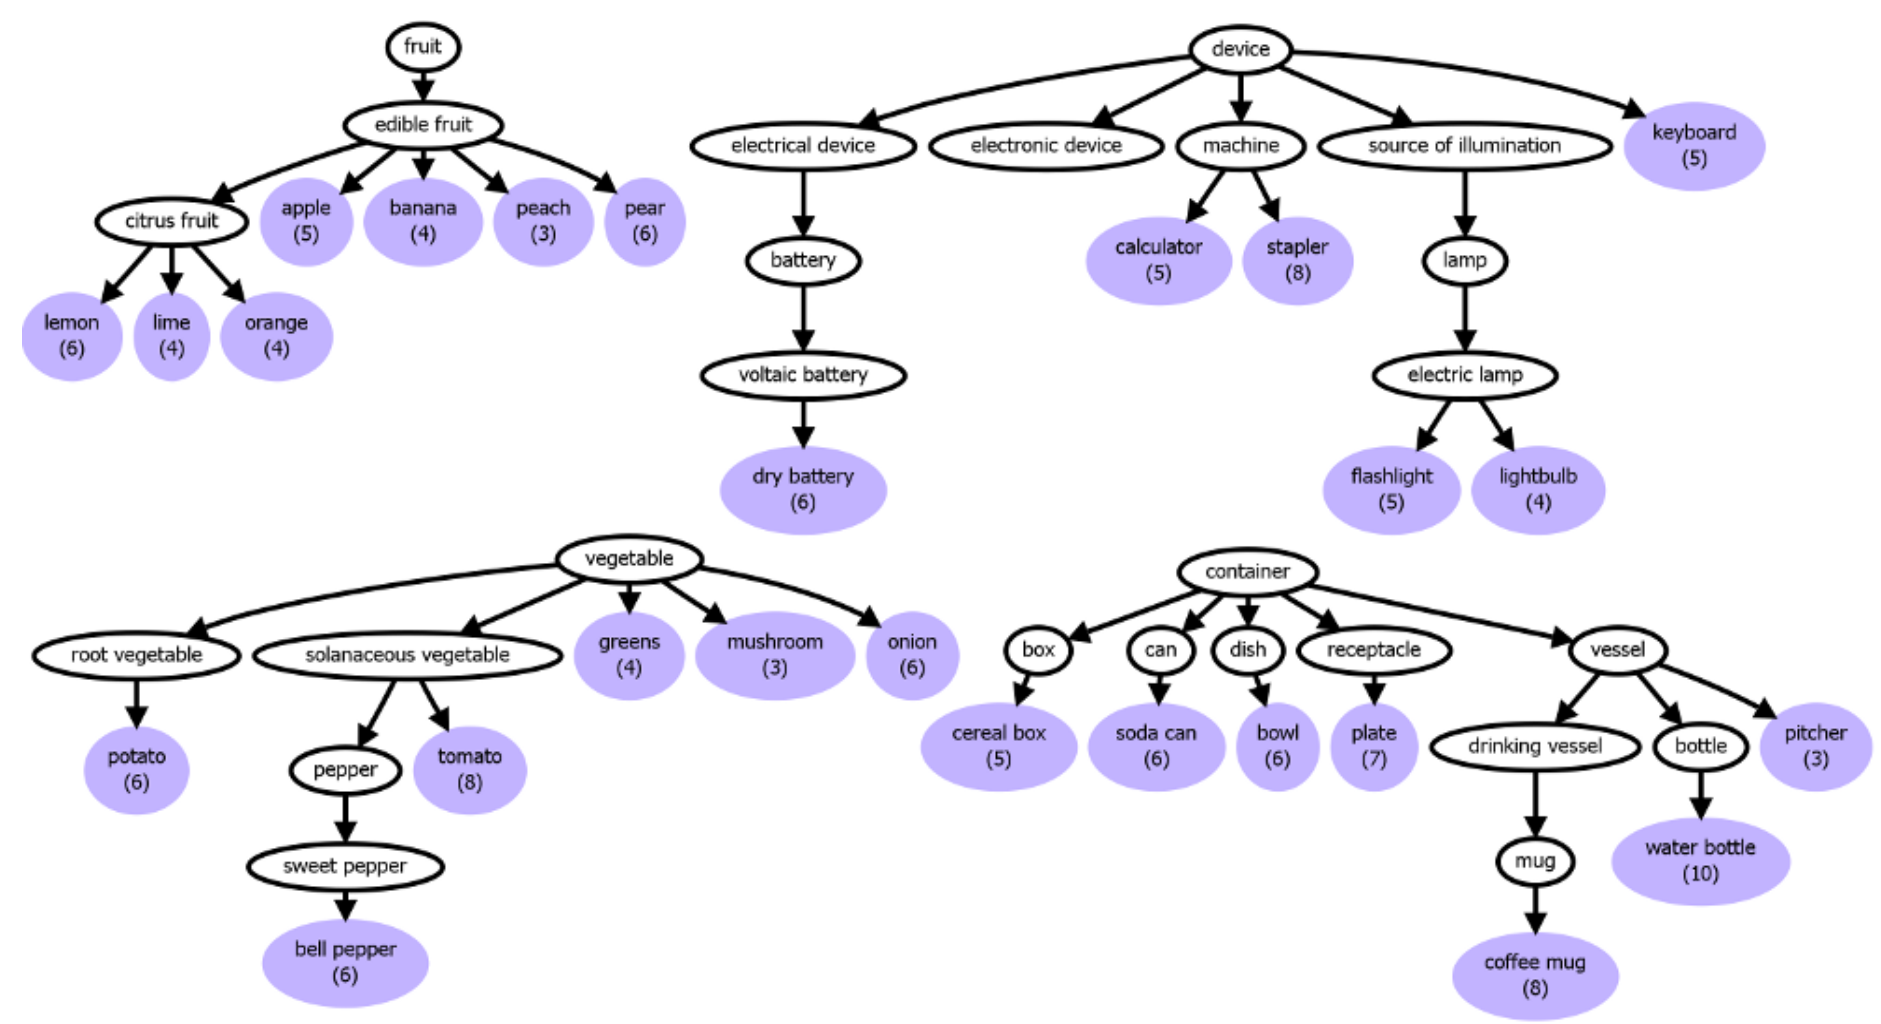
\includegraphics[width=0.9\textwidth]{figure/rgbd}
\caption{Object hierarchy in the dataset as a subset of the ImageNet category. Taken from \cite{dataset}}
\end{figure}
The following figure shows objects from the dataset, where each object belong to a different category. 
\begin{figure}[H]
\centering
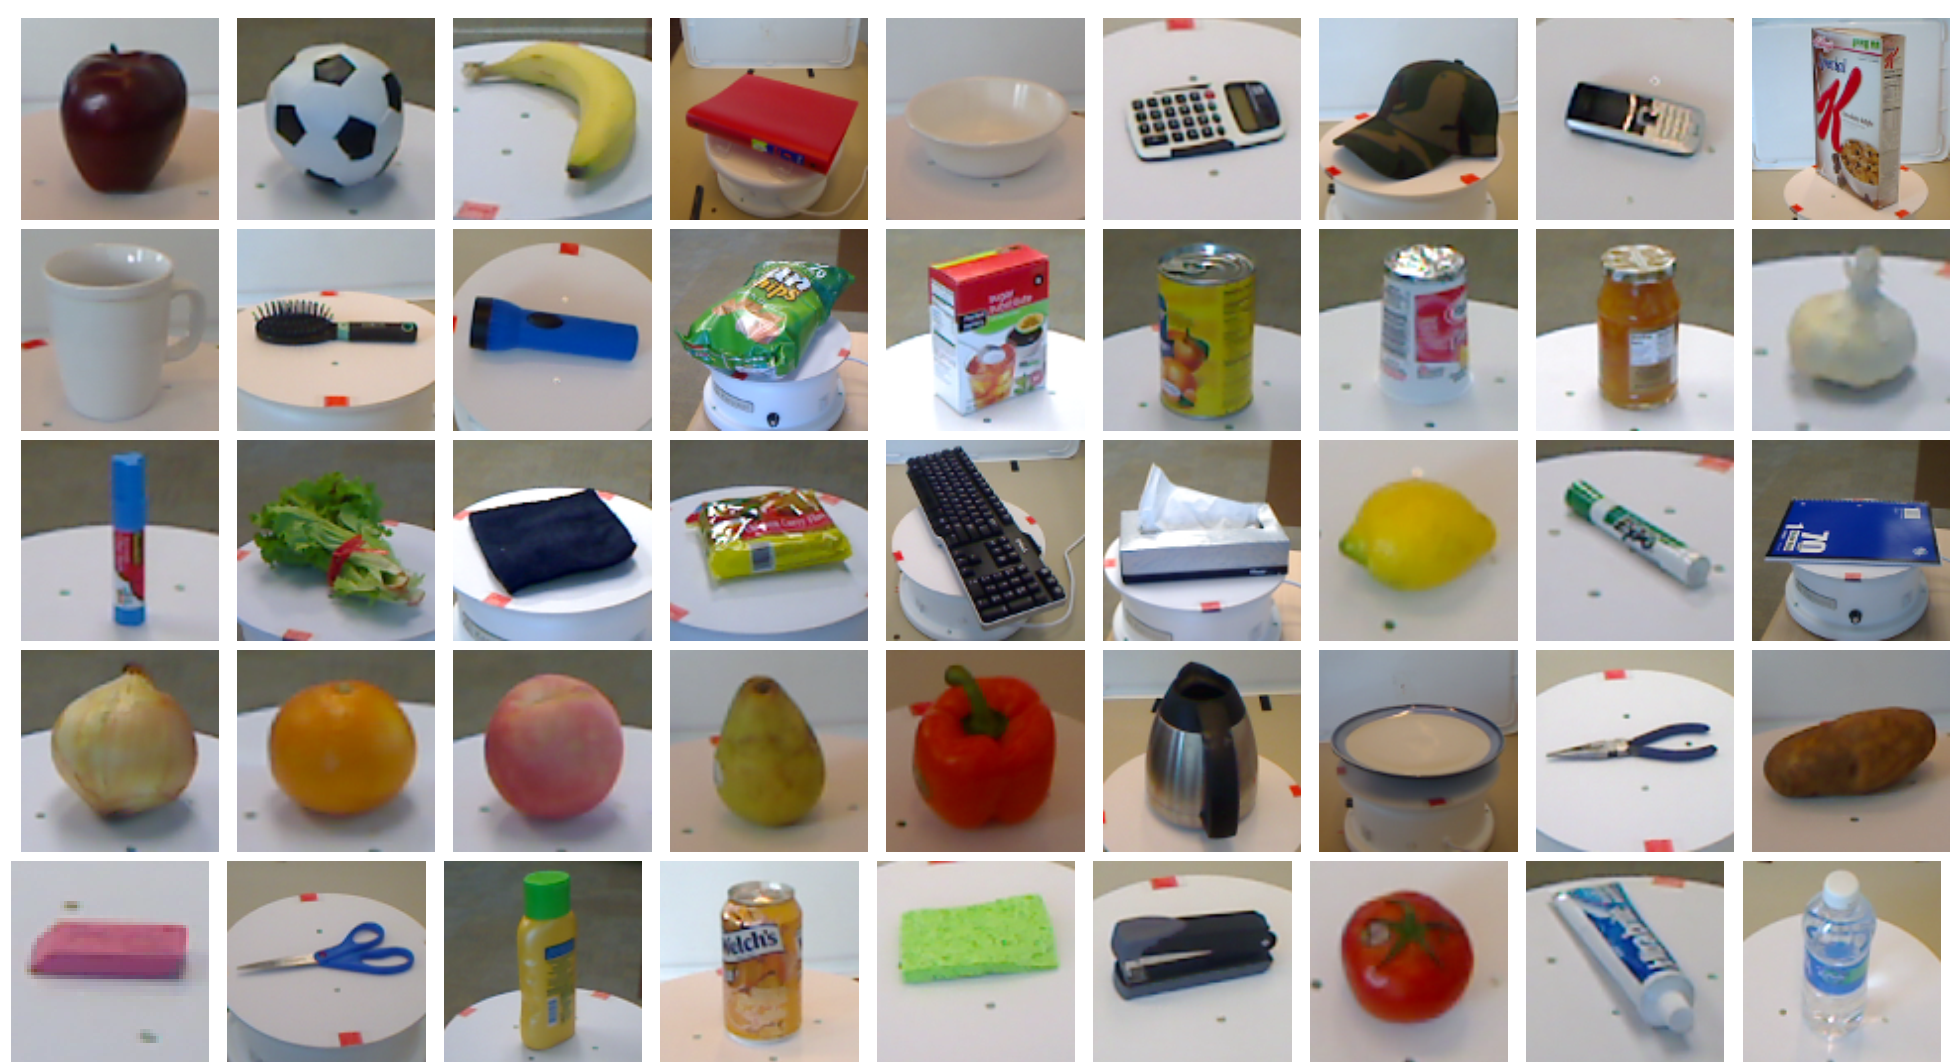
\includegraphics[width=0.7\textwidth]{figure/rgbd1}
\caption{Objects from the RGB-D object dataset. Taken from \cite{lai2011large}}
\end{figure} 
Both of the dataset are created using similar procedure. The video sequence of each object is recorded as the object is spun around a turntable, where cameras mounted at three different heights relative to the turntable, at approximately $30^{\circ}$, $45^{\circ}$ and $60^{\circ}$ above the horizon.
Farther and most importantly, we generate new data using our developed model and use these data to train the model and evaluate the model. 
 


\section{Test procedure}
In this experiment we will reveal, how the accuracy of the classifier increases by a trained model, which contains the data generated from episodic memory.
\\\\For this task, at first we train classifiers on ODU dataset, which contains 8000 samples of 54 objects.The data is produced using the turn table. At this point we test the classifier accuracy with a small dataset contains 480 samples of 25 objects and get the over all classifier accuracy $63 \%$. Each time we test the accuracy of the classifier using different small dataset and in the next step we add this data with the previous trained dataset. The dataset is generated from robot manipulation task.  where each there the new test dataset is the subset of previous test dataset and contains the data of robots manipulation tasks.    At first we test the classifier accuracy using date taken from robot manipulation task in kitchen environment. The test data has 240 samples of 21 objects. Here we get the classifier accuracy is 63%. Then we add the test date to the turn table data. And trained the classiffiers again. This time we use test data, which is taken from another robot manipulation task.  The dataset contains 400 samples of 20 objects and subject of previous test set. At this moment the accuracy of the classifiers increases and the

\begin{figure}[H]
\centering
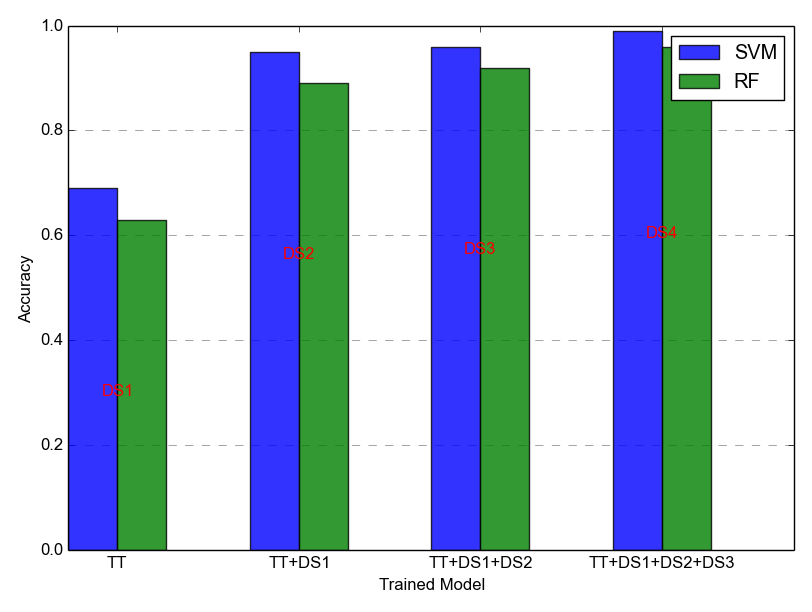
\includegraphics[width=0.9\textwidth]{figure/accu}
\caption{Categorization of WRGBD dataset}
\end{figure}   

\section{Test }
In the first experiment, we will reveal how much train data is needed to get high accuracy of the different classifiers. For this task,  we train classifiers on ODU dataset, which contains 8000 samples of 54 objects. Each time we test the accuracy of the classifier using different small dataset and in the next step we add this data with the previous trained dataset. The dataset is generated from robot manipulation task.  where each there the new test dataset is the subset of previous test dataset and contains the data of robots manipulation tasks.    At first we test the classifier accuracy using date taken from robot manipulation task in kitchen environment. The test data has 240 samples of 21 objects. Here we get the classifier accuracy is 63%. Then we add the test date to the turn table data. And trained the classiffiers again. This time we use test data, which is taken from another robot manipulation task.  The dataset contains 400 samples of 20 objects and subject of previous test set. At this moment the accuracy of the classifiers increases and the accuracy are 80 .
\subsection{Supervised Results}
In this thesis work we consider that the robot is working in the kitchen environment and the task of the robot is like pick and place of the object. We use Washington university dataset \cite{dataset} and kitchen environment dataset from institute for artificial intelligent. Both datasets are created by taken image of different objects using a turn table with and angle difference 30 degree. We use popular supervised machine learning algorithms like support vector machine, random forest, k-nearest neighbor, gradient boost tree to create the trained model in order to classify the data which is coming from real world robot manipulation task. Before classify the real world data we cross validate our trained model using the test data and  evaluate the performance of the classifiers. The real world data is recorded during the robot manipulation task and put it into a database. The real data is row sensor date and consider as unstructured data. 
\subsection{Semi-supervised Results}
  \begin{table}[!htbp]
 \centering 
   \caption{Algorithm's result comparison}
  \rowcolors{2}{gray!25}{green!50}  
  \begin{tabular}{l|c|c|c|c} \hline
  \diaghead{\theadfont Diag ColumnmnHead II}%  
   {Feature+Dataset}{Algorithm}&
  \thead{SVM} &\thead{RF} &\thead{RF} &\thead{GBT} \\ \hline
  BVLC${\_7}$CF + RGBD & foo & bar & foo & bar \\  
  BVLC${\_7}$CF + iai$\_$ODU & foo & bar & foo & bar \\   
  VFH + RGBD & foo & bar & foo & bar \\    
  VFH + iai$\_$ODU & foo & bar & foo & bar \\    
  CVFH + RGBD & foo & bar & foo & bar \\    
  CVFH + iai$\_$ODU & foo & bar & foo & bar \\    
  VGG$16$ + WURGBD & foo & bar & foo & bar \\   
  VGG$16$ + iai$\_$ODU & foo & bar & foo & bar \\    \hline
\end{tabular}

  \end{table}
\chapter{Conclusion}







%%%%%%%%%%%%%%%%%%%%%%%%%%%%%%%%%%%%%%%%%%%%%
%%%  APPENDIX / Anhang                      %
%%%-----------------------------------------%
\begin{appendix}

\chapter{Appendix}
The usages of all the developed softwares are illustrated below.
\\\\
\textbf{Prerequisite:} Robosherlock, Caffe, PCL, openCV, rs{\_}resources
\\\\The \textbf{rs{\_}learning} package consists of three modules.
\begin{itemize}
\item Module for extracting features from image.
\item Module for training the classifier.
\item Module for classify the images. 
\end{itemize}

\section{Extracting Feature Module}
To get help:
\begin{description}
\item[\$] rosrun rs{\_}learning featureExtractor -h
\end{description}
To extract feature             
\begin{description}
\item[\$] rosrun rs{\_}addons featureExtractor -s splitName -i storage -d datasetName 
\\-f feat 
\end{description}
Where:
\begin{description}
\item[splitName] It is a .ymal file, contains informations about objects and object's class label. The file should be in catkin workspace \\ rs{\_}resources/objects{\_}dataset/splits folder.
\item[storage] It is the name of input image storage folder.The folder should be in 
 rs{\_}resources/objects{\_}dataset. For this project we use two datasets, one is  kitchen environment dataset from Institute for Artificial Intelligence and the other one is from Washington University dataset. Parameter's (storage) value should be iaiImageFolder/wuImageFolder, if someone wants to use both datasets at once else just iaiImageFolder or wuImageFolder folder name.
\item[datasetName] It's value should be should be IAI (to use dataset from Institute for 
artificial intelligence) and WU (to use dataset from Washington University). If someone wants to use both datasets at once, he should select the parameter's value as BOTH.
\item[feat] It should be CNN or VGG16 (RGB data) and VFH or CVFH (for RGB-D data).
\end{description}
The above command should generate following files in \\ rs{\_}resources/objects{\_}dataset/extractedFeat folder. So check the folder called extractedFeat is there or not, if not create one and name it as extractedFeat.
\begin{enumerate}
\item datasetName{\_}feat{\_}ClassLabel{\_}splitName.txt 
\item datasetName{\_}feat{\_}MatTrain{\_}splitName.yaml
\item datasetName{\_}feat{\_}MatTrainLabel{\_}splitName.yaml
\item  datasetName{\_}feat{\_}MatTest{\_}splitName.yaml
\item datasetName{\_}feat{\_}MatTestLabel{\_}splitName.yaml
\end{enumerate}

The first file contains the object to class label map in  data type double, second and third file contain the train data and it's label respectively, fourth and fifth file contain test data and it's label accordingly.
\\\\
\textbf{Example:} If someone type the following command:
\begin{description}
\item[\$] rosrun rs{\_}learning featureExtractor -s ObjectOur -i partial{\_}views -d IAI \\ -f CNN
\end{description}
Output should be following:
\begin{enumerate}
\item IAI{\_}CNN{\_}ClassLabel{\_}ObjectOur.txt
\item IAI{\_}CNN{\_}MatTrain{\_}ObjectOur.yaml
\item IAI{\_}CNN{\_}MatTrainLabel{\_}ObjectOur.yaml
\item IAI{\_}CNN{\_}MatTest{\_}ObjectOur.yaml
\item IAI{\_}CNN{\_}MatTestLabel{\_}ObjectOur.yaml
\end{enumerate}
\section{Classifier Trainer Module}
In rs{\_}learning package each annotator has one .xml file in Descriptors/annotators folder and the ensemble of annotators is called analysis engine. If someone wants to 
create the TrainedModel for the specific classifier,should first provide the following parameter's values in trainerAnnotator.xml file.
 
\begin{description}
\item [classifierType] It's value should be rssvm (for support vector mechine) or rsrf (for random forest) or rsgbt (for gradient boost tree) or rsknn (for k-Nearest neighbour).
\item [trainDataName] The name of the train data file \\ (datasetName{\_}feat{\_}MatTrain{\_}ObjectOur) in path \\ rs{\_}resources/objects{\_}dataset/extracetedFeat
\item [train{\_}label{\_}name] The name of the data trainLabel file \\ (datsetName{\_}feat{\_}MatTrainLabel{\_}splitName) in path \\
 rs{\_}resources/objects{\_}dataset/extracetedFeat/ 
\end{description}
It will generate a TrainedModel file as \\ datasetName{\_}feat{\_}classifierTypeModel{\_}ObjectOur.yaml in \\ rs{\_}learning/trainedData folder.
\\\\
\textbf{Example:}
If someone choose parameters classifierType as rssvm, \\ 
trainDataName as IAI{\_}CNN{\_}MatTrain{\_}ObjectOur and \\ train{\_}label{\_}name name as IAI{\_}CNN{\_}MatTrainLabel{\_}ObjectOur in \\ trainerAnnotator.xml file
and type the following command on \\ Ubuntu terminal.
\begin{description}
\item[\$] rosrun robosherlock run model{\_}trainer
\end{description}
Then as output IAI{\_}CNN{\_}rssvmModel{\_}ObjectOur should \\ 
be generated in rs{\_}learning/trainedData folder.

\section{Image Classifier Module}
This module is divided into two parts classify offline and online. 
If someone has test data on hand, he can use ClassifyOffline 
annotator and classifies the images. The command for that:
\begin{description}
\item[\$] rosrun robosherlock run ClassifyOffline
\end{description}
 Before enter the command please tune the following parameter in \\ ClassifyOfflineAnnotator.xml file.

\begin{description}
\item[classifierType] It should be rssvm or rsrf or rsgbt or rsknn
\item[trained{\_}model{\_}name] The name of the trainedModel file (Ex. if 
someone selects classifier{\_}type(= rssvm),then traindModel should 
look like \\ IAI{\_}CNN{\_}rssvmModel{\_}ObjectOur).
\item[test{\_}data{\_}name] It should be the test data file name 
\\(Ex.IAI{\_}CNN{\_}MatTest{\_}ObjectOur.yaml)
\item[test{\_}label{\_}name] The name of the testLabel data file \\(Ex.IAI{\_}CNN{\_}MatTestLabel{\_}ObjectOur)
\item[actual{\_}class{\_}label] The name of classLabel file \\(Ex.IAI{\_}CNN{\_}ClassLabel{\_}ObjectOur)
\end{description}
If the classifier{\_}type (=rsknn), instead of trained{\_}model{\_}name 
selects the following two files.
\begin{description}
\item[trainDatamatrix] The name of the train matrix file 
\\ (Ex.IAI{\_}CNN{\_}MatTrain{\_}ObjectOur)
\item[trainlabel{\_}matrix] The name of the trainLabel matrix file \\(IAI{\_}CNN{\_}MatTrainLabel{\_}ObjectOur)
\end{description}
If test data is coming from a .bag file or any database or from real time robot manipulation task, the process is called online. Then someone has to use the following command.
\begin{description}
\item[\$] rosrun robosherlock run my{\_}demo
\end{description}
my{\_}demo is an analysis engine with many Annotators(specially classifiers). Each classifier has two options. It can classify or set the groundTruth for the images. So before runing the above command please tune the parameters in the respective annotator's .xml file. The parameters name are same for classifiers (rssvm, rsrf, rsgbt) and they are:
\begin{description}
\item[set{\_}mode] It should be CL (to classify) and GT (to set groundtruth )                           
\item[trained{\_}model{\_}name] Name of the trainedModel 
\\(Ex.IAI{\_}CNN{\_}rssvmModel{\_}ObjectOur).
\item[actual{\_}class{\_}label] Name of classLabel file 
\\(Ex.IAI{\_}CNN{\_}ClassLabel{\_}ObjectOur)
\end{description}
And for classifier (rsknn), please selects set{\_}mode (=rsknn) and instead 
of parameter (trained{\_}model{\_}name) tune the the following parameters.
\begin{description}
\item[trainKNN{\_}matrix] The name of the train matrix file 
\\(Ex.IAI{\_}CNN{\_}MatTrain{\_}ObjectOur)
\item[trainKNNLabel{\_}matrix] The name of the trainLabel matrix file \\ (IAI{\_}CNN{\_}MatTrainLabel{\_}ObjectOur)
\end{description}
\textbf{Attention:} When classify images online please make sure that the image features coming from Robosherlock annotators pipeline (Ex. PCLfeatureExtractor or caffe ) must be the same as the respective trainedModel's features.
\end{appendix}




%%%%%%%%%%%%%%%%%%%%%%%%%%%%%%%%%%%%%%%%%%%%%
%%%  Verzeichnisse                          %
%%%-----------------------------------------%


%%% Abbildungsverzeichnis
%\newpage\thispagestyle{empty}{~}\cleardoublepage		% min. eine leere Seite nach Anhang erzwingen
\listoffigures                  % Ausgabe des Abbildungsverzeichnisses


%%% Tabellenverzeichnis
\listoftables			        % Ausgabe des Tabellenverzeichnisses


%%% Literaturverzeichnis
\nocite{*}  % Alle Quellen auflisten / auskommentieren bewirkt,
              % dass nur im Text referenzierte Quellen aufgelistet werden
\bibliography{literatur}{}   % Ausgabe des Literaturverzeichnisses


%%%%%%%%%%%%%%%%%%%%%%%%%%%%%%%%%%%%%%%%%%%%%
%%%%%%%%%%%%%%%%%%%%%%%%%%%%%%%%%%%%%%%%%%%%%
%%%                 %%%%%%%%%%%%%%%%%%%%%%%%%
%%%  Dokument-Ende  %%%%%%%%%%%%%%%%%%%%%%%%%
%%%                 %%%%%%%%%%%%%%%%%%%%%%%%%
%%%%%%%%%%%%%%%%%%%%%%%%%%%%%%%%%%%%%%%%%%%%%
%%%%%%%%%%%%%%%%%%%%%%%%%%%%%%%%%%%%%%%%%%%%%
\end{document}
% EOF 